\documentclass[11pt]{article}
\usepackage[T1]{fontenc}
\usepackage[utf8]{inputenc}
\usepackage{lmodern}
\usepackage[margin=1in]{geometry}
\usepackage{microtype}  % better line breaking + character protrusion

% Global line-break tolerance for long math identifiers
\emergencystretch=2em
\tolerance=1500
\hbadness=10000

% Allow line breaks inside inline math at relation/binary operators
\binoppenalty=700
\relpenalty=500
\usepackage{amsmath,amssymb,amsthm,mathtools,bm,mathrsfs}
\usepackage{longtable,booktabs,array,multirow}
\usepackage{textcomp}
\usepackage{graphicx}
\usepackage{enumitem}
\usepackage{xcolor}
\usepackage{framed}
\usepackage{fancyvrb}
\usepackage{ragged2e}
\usepackage{hyperref}
\usepackage{xurl}
\usepackage{tikz}
\usepackage{tikz-cd}
\usetikzlibrary{arrows.meta, positioning, calc, shapes.geometric, fit, decorations.pathreplacing}
\usepackage{caption}

% Theorem environments
\theoremstyle{plain}
\newtheorem{theorem}{Theorem}[section]
\newtheorem{lemma}[theorem]{Lemma}
\newtheorem{proposition}[theorem]{Proposition}
\newtheorem{corollary}[theorem]{Corollary}

\theoremstyle{definition}
\newtheorem{definition}[theorem]{Definition}
\newtheorem{example}[theorem]{Example}
\newtheorem{remark}[theorem]{Remark}
\newtheorem{convention}[theorem]{Convention}

% Custom commands
\newcommand{\RS}{\mathrm{R\text{-}S}}
\newcommand{\cS}{\mathcal{S}}
\newcommand{\cF}{\mathcal{F}}
\newcommand{\cM}{\mathcal{M}}
\newcommand{\cC}{\mathcal{C}}
\newcommand{\cD}{\mathcal{D}}
\newcommand{\cL}{\mathcal{L}}
\newcommand{\cP}{\mathcal{P}}
\newcommand{\fM}{\mathfrak{M}}
\newcommand{\Meta}{\mathfrak{Meta}}
\newcommand{\LFnd}{\mathcal{L}_{\mathrm{Fnd}}}
\newcommand{\LCls}{\mathcal{L}_{\mathrm{Cls}}}
\newcommand{\LClsMax}{\mathcal{L}_{\mathrm{Cls}}^{\top}}
\newcommand{\LAbs}{\mathcal{L}_{\mathrm{Abs}}}
\newcommand{\gr}{\operatorname{gr}}
\newcommand{\Sint}{\cS_{\mathrm{int}}}
\newcommand{\Ob}{\mathrm{Ob}}
\newcommand{\Mor}{\mathrm{Mor}}
\newcommand{\Hom}{\mathrm{Hom}}
\newcommand{\Fun}{\mathrm{Fun}}
\newcommand{\Cl}{\mathrm{Cl}}
\newcommand{\Lan}{\mathrm{Lan}}
\newcommand{\Ran}{\mathrm{Ran}}
\newcommand{\Set}{\mathrm{Set}}
\newcommand{\Cat}{\mathrm{Cat}}
\newcommand{\Syn}{\mathrm{Syn}}
\newcommand{\Mod}{\mathrm{Mod}}
\newcommand{\Con}{\mathrm{Con}}
\newcommand{\PA}{\mathsf{PA}}
\newcommand{\ZFC}{\mathsf{ZFC}}
\newcommand{\MLTT}{\mathsf{MLTT}}
\newcommand{\HoTT}{\mathsf{HoTT}}
\newcommand{\ETT}{\mathsf{ETT}}
\newcommand{\CIC}{\mathsf{CIC}}
\newcommand{\NBG}{\mathsf{NBG}}
\newcommand{\AFA}{\mathsf{AFA}}
\newcommand{\CZF}{\mathsf{CZF}}
\newcommand{\II}{\mathbf{I}}
\newcommand{\cU}{\mathcal{U}}
\newcommand{\tpi}{\widetilde{\pi}}
\newcommand{\cE}{\mathcal{E}}
\newcommand{\fME}{\fM_{\cE}}
\newcommand{\LAbsE}{\LAbs^{\cE}}
\newcommand{\LClsE}{\LCls^{\cE}}
\newcommand{\LClsMaxE}{(\LClsMax)^{\cE}}
\newcommand{\LFndE}{\LFnd^{\cE}}
\newcommand{\SSE}{\cS_{S}^{\cE}}
\newcommand{\SSEbase}{\cS_{S}^{\cE,\,\mathrm{base}}}
\newcommand{\SSEglobal}{\cS_{S}^{\cE,\,\mathrm{global}}}
\newcommand{\Eff}{\ensuremath{\mathsf{Eff}}}
\newcommand{\OWL}{\ensuremath{\mathsf{OWL}}}
\newcommand{\NCG}{\ensuremath{\mathsf{NCG}}}
\DeclareMathOperator{\colim}{colim}
\DeclareMathOperator{\image}{image}
\DeclareMathOperator{\id}{id}
\DeclareMathOperator{\ev}{ev}
\DeclareMathOperator{\Trace}{Trace}
\DeclareMathOperator{\dep}{depth}

\title{The Moduli Space of Formal Systems:\\
Classification, Stabilization, and a No-Go Theorem for Absolute Foundations}

\author{%
  \footnotesize Max Sereda \\[-3pt]
  \scriptsize\textit{Independent researcher} \\[-3pt]
  \scriptsize\texttt{\href{mailto:max@gst.st}{max@gst.st}}%
}

\date{\scriptsize\today}

\begin{document}
\maketitle

\begin{abstract}
I study the $(\infty, n)$-categorical moduli space $\fM$ of formal systems (hereafter \textbf{MSFS}): the classifying $2$-stack of Morita-equivalence classes of Rich-foundations ($\LFnd$ theories satisfying (R1)--(R5)). I distinguish structural constructions, conditional comparison criteria, open stabilization obligations, and a relative boundary lemma.

\emph{(i) Conditional plurality at $\LCls$.} Classifiers over a common base with distinct essential classification images cannot be equivalent over that base. Applying this criterion to $\infty$-cosmoi, Univalent Foundations, and cohesive frameworks requires explicit classifiers and verification of their images.

\emph{(ii) Conditional meta-categoricity.} Comparison with a common classifier gives a biequivalence when essential surjectivity and equivalences on all hom-categories are supplied. Deriving these lifting conditions from (Max-1)--(Max-4) remains open.

\emph{(iii) Conditional intensional refinement.} A supplied compatible comparison makes a refinement fibre over its chosen base image. An ordinary slice construction exists, but its equivalence-generated display filtration collapses at grade zero. A nontrivial higher refinement and strict Morita separation remain construction problems.

\emph{(iv) Meta-stabilization problem.} Equivalence between iterated classifiers is not established. Fixed-finite-$n$ unicity of higher-category models does not supply it, and unbounded universe ascent requires additional assumptions.

\emph{(v) Conditional AC/OC duality.} At a specified categorical level, a comparison adjunction whose unit is invertible and whose counit is inverted by the chosen localization induces an equivalence after localization. Constructing these data for the proposed theory-centric and enactment-centric moduli, and extending them to unbounded depth, are separate obligations.

\emph{Boundary corollary: the Absolute Foundation No-Go Theorem (AFN-T).} By the syntax--semantics adjunction underlying (R5), the defined $\LAbs$ stratum (formally definable, non-reducible, and maximally generative foundation) is empty. AFN-T subsumes the classical no-go series Cantor~\cite{Cantor1891}, Russell~\cite{Russell1903}, G\"odel~\cite{Godel1931}, Tarski~\cite{Tarski1936}, Lawvere~\cite{Lawvere1969}, Ernst~\cite{Ernst2015} uniformly across $\RS$ and all $(\infty, n)$, $n \in \mathbb{N} \cup \{\infty\}$, and extends dually to the enactment-absolute stratum $\LAbs^\cE$.

\smallskip
\noindent\textbf{Keywords:} moduli space of formal systems, classifying $2$-stacks, categorical logic, $(\infty, n)$-categories, higher topos theory, intensional type theory, meta-classification, effective topos, no-go theorems.

\smallskip
\noindent\textbf{MSC2020:} 03A05, 03B30, 03C45, 03F40, 18A05, 18N10, 18N50, 18N60, 18N65.

\end{abstract}

\newpage
\tableofcontents
\newpage

\section{Introduction}

\paragraph{Scope audit (8 October 2026).}
AFN-T's identity argument is relative to the defined class $\cS_S$ and
the definition of $\Pi_4$. It does not exclude new mathematics, new
foundations, or operational refinements of Morita-equivalent realizations.
In particular, a cost/time invariant descends through a localization only
if it sends every inverted morphism to an equivalence. The reflective
localization used for enactments does not automatically retain execution
cost, causality, memory, or production resources. An Autogeny realization
therefore requires these data above the localized classifier and separate
proofs that its interpretation preserves them.



This paper studies the \emph{moduli space of formal systems} $\fM$, the classifying $(\infty, 2)$-stack whose points are Morita-equivalence classes of Rich-foundations (formal theories $F$ satisfying conditions (R1)--(R5) of Definition~\ref{def:rs}) and whose $k$-morphisms are faithful interpretations and provable natural equivalences. The principal results concern the structure of $\fM$:
\begin{itemize}
\item \textbf{Stratification} (\S\ref{sec:hierarchy}): $\LFnd \xrightarrow{\mathrm{Cls}} \LCls \supseteq \LClsMax \xrightarrow{\mathrm{Gen}} \LAbs = \emptyset$ --- the strata are cut out by type-distinct condition packages ((R1)--(R5) on formal systems vs.\ (M1)--(M5) on classifiers, Proposition~\ref{prop:level-structure}~(ii)); the sole inclusion is $\LClsMax \subseteq \LCls$.
\item \textbf{Conditional structural plurality at $\LCls$} (Theorem~\ref{thm:meta-mult}).
\item \textbf{Conditional categoricity of $\LClsMax$} (Theorem~\ref{thm:meta-cat}).
\item \textbf{Open meta-stabilization and universe obligations} (Remark~\ref{thm:meta-stab}).
\item \textbf{Conditional slice-locality} (Theorem~\ref{thm:slice-locality}), requiring a supplied compatible comparison.
\item \textbf{Generated filtrations and their limitation} (Definition~\ref{def:display-grade}, Proposition~\ref{prop:grading}): generator-preserving functors cannot increase grade; the former equivalence-only seed gives grade zero everywhere (Corollary~\ref{cor:grade-collapse}).
\item \textbf{Five-axis absoluteness} (\S\ref{sec:five-axis}).
\item \textbf{Conditional AC/OC comparison} (Theorem~\ref{thm:ac-oc-duality}); the separate relative identity obstruction is Theorem~\ref{thm:dual-afnt}.
\item \textbf{Outer boundary: $\LAbs = \emptyset$} --- the Absolute Foundation No-Go Theorem (Theorem~\ref{thm:afnt-alpha}, Theorem~\ref{thm:afnt-beta}).
\end{itemize}

\paragraph{Machine verification.} The companion Verum corpus must be replayed against the exact claims and assumptions of this revision. The current paper does not certify machine-checked coverage of every statement; see the verification ledger in Appendix~\ref{app:verification-ledger}.

\subsection{Notation and Conventions}

\begin{convention}\label{conv:zfc-inacc}
I work throughout in $\ZFC$ augmented by two inaccessible cardinals $\kappa_1 < \kappa_2$, providing Grothendieck universes $\mathbf{U}_1 \subset \mathbf{U}_2$ sufficient for the $2$-categorical machinery used. The categorical machinery follows Kelly~\cite{Kelly1982} for enriched and $2$-categories, Lurie~\cite{LurieHTT} for $(\infty, 1)$-categories, Lurie~\cite{LurieHA} for higher algebra, and Riehl--Verity~\cite{RiehlVerity2022} for $\infty$-cosmoi. For accessible functor theory I follow Ad\'amek--Rosick\'y~\cite{AdamekRosicky1994}.
\end{convention}

\begin{convention}[Key symbols]\label{conv:notation}
\begin{itemize}
\item $\cF$ denotes the $2$-category of \emph{Rich-foundations} ($\LFnd$): objects are foundational theories in the sense formalised in \S\ref{sec:rs} below (conditions (R1)--(R5)); $1$-morphisms are faithful interpretations; $2$-morphisms are provable natural equivalences between interpretations.
\item $\rho : \cF \to (\infty, n)\text{-}\Cat$ denotes the \emph{classification functor} assigning to each $F \in \cF$ its category of models (or, for type-theoretic $F$, the syntactic $(\infty, n)$-category $\Syn(F)$).
\item A \emph{gauge transformation} $\tau : F_1 \to F_2$ is a $1$-morphism in $\cF$ accompanied by a distinguished $2$-equivalence $\rho(F_1) \simeq \rho(F_2)$ at the model-categorical level. Two foundations are \emph{gauge-equivalent} if there is an invertible gauge transformation between them. \emph{Relation to Morita equivalence.} Gauge-equivalence at the $\cF$-level corresponds, via the $\fM := \cF/\text{gauge}$ quotient, to Morita equivalence at the stack level: $F_1, F_2 \in \cF$ are gauge-equivalent iff $[F_1] = [F_2]$ in $\fM$, which by construction is the Morita-equivalence class. Throughout the paper, ``gauge'' (1-morphism level) and ``Morita'' (stack level) name the same underlying equivalence relation at their respective categorical strata, related by the $\cF \to \fM$ quotient functor; no distinct third relation is introduced.
\item \emph{Morita-reducibility at the $(\infty, n)$-level}: a $\LAbs$ candidate $X$ and any $Y \in \cS_S$ are each viewed as pointed $(\infty, n)$-categorical structures via the canonical Yoneda embedding into the total $(\infty, n)$-category $\mathbf{StrCat}_{S, n}$ of $S$-structured $(\infty, n)$-categories (Definition~\ref{def:strcat}, stated immediately below). Concretely, $X$ presented by a formula $\phi_X$ corresponds to the pair $(\Syn(S), [\phi_X])$ where $[\phi_X]$ is the isomorphism class of the object defined by $\phi_X$ in the syntactic category; $Y \in \Ob(\cM) \subseteq \cS_S^{\mathrm{local}}$ corresponds to $(\cM, Y)$. I write $X \to_{M, n} Y$, and say $X$ is \emph{Morita-reducible at the $(\infty, n)$-level} to $Y$, if there exists an $(\infty, n)$-functor $\Phi : \Syn(S) \to \cM$ in $\mathbf{StrCat}_{S, n}$ sending $[\phi_X]$ to the isomorphism class of $Y$, with the restriction $\Phi |_{[\phi_X]}$ an $(\infty, n)$-equivalence onto its image. This extends classical ring-Morita equivalence (which compares $\Mod(X)$ and $\Mod(Y)$ as $1$-categories) by incorporating the full $(\infty, n)$-categorical structure; the two notions coincide when $X, Y$ are $1$-categorical and $n = 1$. I use the shorthand ``Morita-equivalent'' for the symmetric notion and ``Morita-reducible'' for the directed version.
\item $\fM$ denotes the \emph{classifying $2$-stack} of $\cF$: the quotient $\fM := \cF / \text{gauge}$, regarded as an $(\infty, 2)$-stack of Morita-equivalence classes of Rich-foundations. Formally, $\fM$ is the straightening of the Cartesian fibration $\int \rho \to \mathrm{R\text{-}S}$ whose fiber over $S$ is the $2$-groupoid $\rho^{-1}(S)$ of foundations over $S$ modulo gauge. The construction follows Lurie HTT~\cite{LurieHTT} \S 3.2 (straightening--unstraightening of Cartesian fibrations).
\item For a $2$-category $\mathbf{F}$, $\mathrm{Aut}_2(\mathbf{F})$ denotes the $2$-group of $2$-autoequivalences $\mathbf{F} \xrightarrow{\simeq_2} \mathbf{F}$ (monoidal under composition, with invertible $1$-morphisms and coherent $2$-cells).
\item $\Sint$ denotes the $2$-category of display $2$-categories (rigorous definition deferred to Appendix~\ref{app:categorical} below).
\item All $2$-categories are locally small and $\kappa_1$-accessible unless stated otherwise. (For specific Rich-foundations $S$ whose consistency strength requires the second inaccessible, the $\Syn(S)$-accessibility parameter generalizes to $\kappa_S \in \{\kappa_1, \kappa_2\}$ per the accessibility clause (R5a) of the Rich-metatheory definition, formalised in \S\ref{sec:rs} below; subsequent $\kappa_1$-statements should be read uniformly as $\kappa_S$-statements where $S$ is indexed by the specific $\LFnd$-point under consideration. All proofs in this paper are stable under this uniform reading, since the accessibility arguments invoke only regularity of the cardinal, not its specific value.)
\item \emph{Truncation and comparison across depths}: $\Syn^{(\infty,n)}(S)$ denotes a presentation in an explicitly chosen model at depth $n$, when such a presentation and its comparison maps have been supplied. Changing depth requires functors with stated universal properties and coherent transition maps; a reference to left Kan extension alone does not construct a lift of a single syntactic category. The notation $n=\infty$ requires a separately specified unbounded-depth model. No equality of this model with an unspecified colimit, or stabilization under enrichment, is assumed.
\end{itemize}
\end{convention}

\begin{definition}[The total $(\infty, n)$-category $\mathbf{StrCat}_{S, n}$]\label{def:strcat}
For $S \in \RS$ and $n \in \mathbb{N} \cup \{\infty\}$, the \emph{total $(\infty, n)$-category of $S$-structured $(\infty, n)$-categories}, denoted $\mathbf{StrCat}_{S, n}$, has:
\begin{itemize}
\item \textbf{Objects}: pairs $(\cC, \mathrm{str}_\cC)$ where $\cC$ is an $(\infty, n)$-category that is either essentially $\mathbf{U}_1$-small or $\kappa_1$-accessible (the two cases cover syntactic categories and model categories respectively; cf.\ (R5a)) and $\mathrm{str}_\cC$ is an $S$-model structure on $\cC$ (i.e., an interpretation of $S$-signature into $\cC$ satisfying the axioms of $S$).
\item \textbf{$1$-morphisms}: $S$-preserving $(\infty, n)$-functors $\Phi : (\cC_1, \mathrm{str}_1) \to (\cC_2, \mathrm{str}_2)$, i.e., functors commuting with the respective $S$-model structures up to coherent $(\infty, n)$-isomorphism.
\item \textbf{Higher morphisms}: coherent $(\infty, n)$-natural transformations between $S$-preserving functors.
\end{itemize}
I embed objects of $\Syn(S)$ and of any model $\cM \models S$ into $\mathbf{StrCat}_{S, n}$ via the pointing construction $X \mapsto (\Syn(S), X)$ and $Y \mapsto (\cM, Y)$ respectively. Morita-reducibility, as specified in Convention~\ref{conv:notation}, refers to the existence of an $S$-preserving $(\infty, n)$-functor in $\mathbf{StrCat}_{S, n}$ between such pointed structures that is an equivalence onto its image.
\end{definition}

\subsection{Assumption Register}\label{sec:assumption-register}

The register distinguishes the metatheoretic base, structural definitions, and additional hypotheses of conditional results. In particular, the comparison criterion does not derive categoricity from (Max-1)--(Max-4), and the proposed meta-stabilization is open. Downstream uses must check the hypotheses of the cited statement rather than infer proved status from a theorem number.

\begin{description}
\item[\textbf{(A1) Foundational base.}] $\ZFC$ plus two strongly inaccessible cardinals $\kappa_1<\kappa_2$ (Convention~\ref{conv:zfc-inacc}). \emph{Status: foundational axiom package.} This is the declared base for constructions whose size and existence conditions have been verified. It does not certify its own consistency. A model construction gives an upper consistency bound; equiconsistency requires a converse interpretation or a separate lower-bound argument.
\item[\textbf{(A2) Scope of ``metatheory''.}] The no-go quantifies over $\RS$ as delimited by (R1)--(R5) (\S\ref{sec:rs}): recursively enumerable, interpreting Robinson's $Q$, possessing a model in $\mathbf{U}_2$, $\mathbf{StrCat}$-compatible, with essentially $\mathbf{U}_1$-small $\Syn(S)$ of $\kappa_S$-accessible $\mathrm{Ind}$-completion (R5a). \emph{Status: definitional scope.} Systems outside $\RS$ --- non-r.e.\ oracle theories, infinitary logics without accessible syntax --- are not ruled on. Theorem~\ref{thm:afnt-alpha} is universal over $\RS$, not over an informal totality of ``all foundations''.
\item[\textbf{(A3) Formal content of ``absolute foundation''.}] $\LAbs$ membership is \emph{defined} as the conjunction $(F_S) \wedge (\Pi_{4, S, n}) \wedge (\Pi_{3\text{-max}, S, n})$ (Definition~\ref{def:level6}). \emph{Status: interpretive adequacy assumption.} AFN-T forecloses precisely this triple; the philosophical reading ``no absolute foundation exists'' is faithful exactly to the extent the triple captures the intended notion. The five-axis analysis of \S\ref{sec:five-axis} hardens this reading axis-by-axis but does not eliminate its interpretive character.
\item[\textbf{(A4) Comparison relation.}] Objects are compared through Morita-reducibility: existence of an $S$-preserving $(\infty, n)$-functor in $\mathbf{StrCat}_{S, n}$ that is an equivalence onto its image, with objects embedded by the pointing construction (Definition~\ref{def:strcat}). \emph{Status: structural convention.} A finer or coarser comparison topology would redraw stratum boundaries; \S\ref{sec:intensional-grading} measures exactly what the Morita quotient forgets.
\item[\textbf{(A5) Axis exhaustiveness.}] The escape-parameter space is taken to be the five axes $(S, n, \mu, \xi, \pi)$ of \S\ref{sec:five-axis}. \emph{Status: definitional scope, not a theorem.} Exhaustiveness holds by definition of what the paper counts as an escape parameter; a genuinely new axis would require a new theorem, not contradict an existing one.
\item[\textbf{(A6) Meta-classifier axioms.}] The proposed classifying apparatus satisfies (M1)--(M5) and, for the maximal class, (Max-1)--(Max-4). \emph{Status: axioms on a proposed classifier.} The joint-separation clause of (Max-4) supplies neither morphism lifts nor equivalences on hom-categories. Theorem~\ref{thm:meta-cat} additionally requires comparison functors that are essentially surjective and locally equivalences. Existence of these data remains open.
\item[\textbf{(A7) Localization semantics of equivalence.}] The AC/OC duality (\S\ref{sec:ac-oc-duality}) reads ``equivalence'' through $\mathrm{gauge}_\cE$, the $2$-localization of $\cE$ at the reflection morphisms $\mathcal{R}_\cE$ (Pronk calculus of fractions, (BF1)--(BF5)): the reflection unit is inverted \emph{by} the localization, never in $\cE$ itself. \emph{Status: semantic convention}, of the same kind as ring-theoretic Morita equivalence.
\item[\textbf{(A8) Display generators.}] A filtration requires specified seeds and allowed operations. \emph{Status: presentation data.} The formerly canonical seed of equivalences produces a constant filtration. Nontrivial syntactic or resource-sensitive generators and invariance under their comparison maps are additional obligations.
\end{description}

\begin{remark}[Interface for limiting extensions]\label{rem:register-interface}
The register is an interface for extensions: each extension must specify which assumptions it inherits and which it replaces. An extension may require a stronger base; neither an upper bound nor equiconsistency follows from naming the base. AFN-T excludes the explicitly defined $\LAbs$ conjunction within its stated definability scope. It does not prove consistency of other proposed extensions, categoricity of a maximal classifier, or a bound on future mathematical constructions.
\end{remark}

\section{Stratified Hierarchy of the Moduli Space}\label{sec:hierarchy}

I stratify $\fM$ into four formal strata distinguished by the two structurally distinct meta-operations $\mathrm{Cls}$ (horizontal, classifying) and $\mathrm{Gen}$ (vertical, generative). The strata, defined by their categorical conditions, are:
\[
\LFnd \;\xrightarrow{\mathrm{Cls}}\; \LCls \;\supsetneq\; \LClsMax \;\xrightarrow{\mathrm{Gen}}\; \LAbs.
\]

\begin{figure}[ht]
\centering
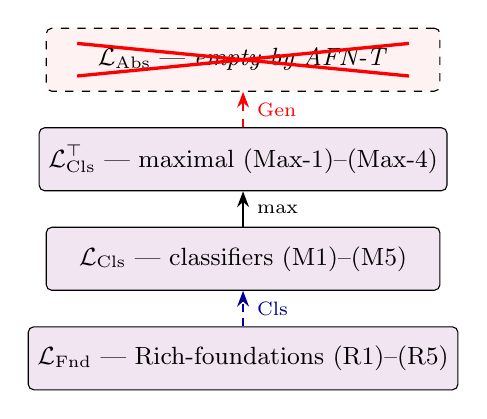
\begin{tikzpicture}[
  level/.style={draw, rounded corners=2pt, minimum width=5cm, minimum height=0.8cm, align=center, font=\small},
  bluefill/.style={fill=blue!6},
  violetfill/.style={fill=violet!10},
  emptybox/.style={draw, dashed, rounded corners=2pt, minimum width=5cm, minimum height=0.8cm, align=center, font=\small, fill=red!5},
  novelty/.style={-{Stealth[length=2mm]}, thick},
  horizmeta/.style={-{Stealth[length=2mm]}, thick, blue!60!black, densely dashed},
  vertmeta/.style={-{Stealth[length=2mm]}, thick, red, dashed},
  node distance=0.45cm
]
\node[level, violetfill] (L5) {$\LFnd$ --- Rich-foundations (R1)--(R5)};
\node[level, violetfill, above=of L5] (L5plus) {$\LCls$ --- classifiers (M1)--(M5)};
\node[level, violetfill, above=of L5plus] (L5max) {$\LClsMax$ --- maximal (Max-1)--(Max-4)};
\node[emptybox, above=of L5max] (L6) {$\LAbs$ --- \emph{empty by AFN-T}};
\draw[horizmeta] (L5.north) -- (L5plus.south) node[midway, right, font=\scriptsize, blue!60!black] {$\,\mathrm{Cls}$};
\draw[novelty] (L5plus.north) -- (L5max.south) node[midway, right, font=\scriptsize] {$\,\mathrm{max}$};
\draw[vertmeta] (L5max.north) -- (L6.south) node[midway, right, font=\scriptsize, red] {$\,\mathrm{Gen}$};
\draw[red, very thick] ($(L6.north west)+(0.4,-0.2)$) -- ($(L6.south east)+(-0.4,0.2)$);
\draw[red, very thick] ($(L6.north east)+(-0.4,-0.2)$) -- ($(L6.south west)+(0.4,0.2)$);
\end{tikzpicture}
\caption{The proposed formal stratification of $\fM$. Classification and maximal generation are distinct operations. The maximality conditions define $\LClsMax\subseteq\LCls$; they do not by themselves prove categoricity, existence of maximal classifiers, or strictness of the inclusion. The relative AFN-T argument excludes the explicitly defined $\LAbs$ conjunction. Any transport to enactment-centric moduli is conditional on the comparison and localization data of Theorem~\ref{thm:ac-oc-duality}.}
\label{fig:hierarchy}
\end{figure}

\subsection{The Formal Strata}

\begin{definition}[Stratified hierarchy --- formal]\label{def:hierarchy}
I define the formal \emph{strata} as classes of mathematical objects:

\begin{tabular}{@{}ll@{}}
\toprule
Class & Membership criterion \\ \midrule
$\LFnd$ & Formal systems satisfying (R1)--(R5) (specified in \S\ref{sec:rs} below) \\
$\LCls$ & Classifiers satisfying (M1)--(M5) (specified in \S\ref{sec:meta} below) \\
$\LClsMax$ & Classifiers additionally satisfying (Max-1)--(Max-4) (specified in \S\ref{sec:meta} below) \\
$\LAbs$ & Objects satisfying $(F_S) \wedge (\Pi_{4, S, n}) \wedge (\Pi_{3\text{-max}, S, n})$ for some $(S, n)$ (specified in \S\ref{sec:conditions} below) \\
\bottomrule
\end{tabular}
\end{definition}

\begin{proposition}[Structural properties of the hierarchy]\label{prop:level-structure}
\begin{enumerate}
\item[\textbf{(i)}] \emph{Definability.} Each of the four strata is a (possibly proper) class definable in $\ZFC + 2\text{-inacc}$ augmented by the $2$-categorical machinery of Convention~\ref{conv:zfc-inacc}. For $\LFnd$ the conditions are (R1)--(R5) (\S\ref{sec:rs} below); for $\LCls$ they are (M1)--(M5) (\S\ref{sec:meta} below); for $\LClsMax$ they strengthen to (Max-1)--(Max-4) (\S\ref{sec:meta} below); $\LAbs$ is defined by the triple $(F_S) \wedge (\Pi_{4, S, n}) \wedge (\Pi_{3\text{-max}, S, n})$ for some $(S, n)$ (\S\ref{sec:conditions} below; the structural self-contradiction of this triple, recorded in \S\ref{sec:afnt-alpha}, yields Theorem~\ref{thm:afnt-alpha}).
\item[\textbf{(ii)}] \emph{Multi-stratum membership.} $\LFnd$ and $\LCls$ concern different data: a formal theory and a specified classifier. A constructed object carrying both structures can satisfy both condition packages. No such membership is inferred solely from the name of a research programme.
\item[\textbf{(iii)}] \emph{Inclusion at the maximal layer.} $\LClsMax\subseteq\LCls$. Strictness requires a constructed classifier failing at least one maximality condition. Theorem~\ref{thm:meta-cat} is a conditional biequivalence criterion with additional comparison data, and Theorem~\ref{thm:meta-mult} gives a conditional image-separation criterion; neither constructs the proposed witnesses.
\item[\textbf{(iv)}] \emph{Emptiness of the absolute stratum.} $\LAbs = \emptyset$ by Theorem~\ref{thm:afnt-alpha}. Consequently $\LFnd \cap \LAbs = \LCls \cap \LAbs = \LClsMax \cap \LAbs = \emptyset$ trivially.
\end{enumerate}
\end{proposition}

\begin{proof}
\textbf{(i)} Each criterion is first-order-expressible; the specified classes are definable.

\textbf{(ii)} The condition sets concern disjoint aspects of an object: axioms with proof calculus vs.\ $2$-categorical structure with classifying functor. An object carrying both structures satisfies both criteria simultaneously.

\textbf{(iii)} Inclusion follows because (Max-1)--(Max-4) strengthen (M1)--(M5). Neither strictness nor equivalence of maximal classifiers follows from this implication alone.

\textbf{(iv)} Immediate from Theorem~\ref{thm:afnt-alpha}.
\end{proof}

\subsection{Examples}

\paragraph{Stratum $\LFnd$.} Foundations, with characteristic features:

\begin{longtable}{@{}p{3.8cm}l p{4cm} p{4.6cm}@{}}
\toprule
Foundation & Year & Originator & Characteristic \\ \midrule
Z (Zermelo) & 1908 & Zermelo & No Replacement \\
ZF/ZFC & 1922 & Zermelo, Fraenkel & Classical set theory \\
ZFC + inacc & 1963+ & Grothendieck & With universes \\
NBG & 1925--40 & von Neumann, Bernays, G\"odel & First-class classes \\
MK & 1955 & Morse, Kelley & Impredicative classes \\
KP/KPU & 1965 & Kripke--Platek & Admissible sets \\
ETCS & 1964 & Lawvere & Elementary category of sets \\
ETCC & 1966 & Lawvere & Elementary theory of categories \\
NF; NFU & 1937; 1969 & Quine; Jensen & Stratified comprehension \\
CZF & 1978 & Aczel & Constructive ZF \\
IZF & 1970s & Friedman & Intuitionistic ZF \\
PA & 1889 & Peano & First-order arithmetic \\
$\mathsf{Z}_2$ & 20c & Hilbert--Bernays & Second-order arithmetic \\
MLTT & 1984 & Martin-L\"of & Dependent types \\
CIC & 1988--90 & Coquand--Huet; Coquand--Paulin & Inductive constructions \\
HoTT & 2005+ & Awodey, Voevodsky & Univalence + identity types \\
Cubical HoTT & 2015+ & Cohen--Coquand et al. & Computational univalence \\
Universe-poly.\ HoTT & 2013+ & Voevodsky & Universe polymorphism \\
Linear logic + ! & 1987 & Girard & Resource-sensitive \\
NBG + AFA & 1988 & Aczel & Non-well-founded sets \\
$(\infty, 1)$-topos theory & 2009 & Lurie & $(\infty, 1)$-topoi \\
Non-commutative geom.\ & 1980s & Connes & Spectral triples \\
Cohesive $(\infty, 1)$-topos & 2013 & Schreiber & Cohesion modalities \\
Motivic $\mathrm{SH}(k)$ & 1999 & Voevodsky, Morel & Motivic homotopy \\
Realizability (Eff) & 1982 & Hyland & Effective topos \\
Markov constructive math & 1950s--1980s & A.A.~Markov, Nagornyj & Constructive analysis + Markov's principle \\
Bishop constructive analysis & 1967 & Bishop, Bridges & Choice-free constructive real analysis \\
Synthetic diff.~geom.\ & 1970s & Kock, Lawvere & Infinitesimals as axioms \\
Elementary higher topos & 2021 & Rasekh & Elementary $(\infty, 1)$-topos \\
\bottomrule
\end{longtable}

\paragraph{Stratum $\LCls$.} Classifiers (meta-frameworks). The conditions partition this proposed class into $\Meta_{\mathrm{Cls}}^{\top}$ and its complement. The following programmes motivate candidate classifiers; their names alone do not specify objects satisfying (M1)--(M5). Categoricity requires the comparison hypotheses of Theorem~\ref{thm:meta-cat}.

\begin{longtable}{@{}p{3.3cm}l p{3cm} p{4.4cm}c@{}}
\toprule
Meta-framework & Year & Originator & Classification focus & In $\Meta_{\mathrm{Cls}}^{\top}$? \\ \midrule
$\infty$-cosmoi & 2022 & Riehl--Verity & $(\infty, 1)$-categorical theories & Open \\
Univalent Foundations & 2010+ & Voevodsky & HoTT extensions & Open \\
Cohesive framework & 2013 & Schreiber & Cohesive $\infty$-topoi & Open \\
Higher Algebra prog.\ & 2017+ & Lurie & Stable $\infty$-cat + operadic & Open \\
Synthetic mathematics & 2000s+ & Taylor, Shulman & Axiomatic synthetic foundations & Open \\
\bottomrule
\end{longtable}

\paragraph{Stratum $\LAbs$.} Empty, by AFN-T.

\subsection{The Two Meta-Operations}\label{sec:indexing-scheme}

\paragraph{Horizontal and vertical meta.} Two categorically distinct meta-operations act on a stratum $\mathcal{L}$:
\begin{itemize}
\item \textbf{Horizontal (classifying) meta.} $\mathrm{Cls}(\mathcal{L})$ is the class of $2$-categories $\mathbf{F}$ \emph{classifying} but not \emph{generating} members of $\mathcal{L}$: locally small, equipped with an accessible classification functor into the moduli of $\mathcal{L}$, non-generative, and metatheory-parametrized (cf.\ (M1)--(M5)).
\item \textbf{Vertical (generative) meta.} $\mathrm{Gen}(\mathcal{L})$ is the class of frameworks \emph{generating} members of $\mathcal{L}$ as internal derivations --- candidate absolute foundations.
\end{itemize}

\begin{proposition}[Non-collapse of the horizontal meta at $\LFnd$]\label{prop:no-collapse}
$\mathrm{Cls}(\LFnd)$ does \emph{not} embed into $\LFnd$ and does not coincide with $\LAbs$. It is therefore a distinct formal stratum, which I label $\LCls$.
\end{proposition}

\begin{proof}[Proof sketch.]
A member $\mathbf{F} \in \mathrm{Cls}(\LFnd)$ is a $2$-category of Rich-foundations with an accessible classification functor into $\fM$. It is not itself a Rich-foundation (it does not satisfy (R1)--(R5) for a generating theory), so $\mathbf{F} \notin \LFnd$. It is not in $\LAbs$ because (M4) requires non-generativity, while $\LAbs$ requires maximal generativity $(\Pi_{3\text{-max}})$.
\end{proof}

\paragraph{Horizontal stabilization.} Equivalence of iterated classifiers is an open problem (Remark~\ref{thm:meta-stab}); AFN-T does not prove that no further classifier structure can arise.

\paragraph{Vertical step to the forbidden stratum.} $\LAbs \supseteq \mathrm{Gen}(\LFnd)$: a member of $\LAbs$ would be a maximally-generative foundation from which all of $\LFnd$ derives. This is categorically a fresh operation, not an iteration of $\mathrm{Cls}$. By AFN-T, $\LAbs = \emptyset$.

\paragraph{Summary.} The formal sequence reads:
\[
\underbrace{\LFnd}_{\text{(R1)--(R5)}} \; \xrightarrow{\mathrm{Cls}} \; \underbrace{\LCls}_{\text{(M1)--(M5)}} \; \supsetneq \; \underbrace{\LClsMax}_{(\mathrm{Max}\text{-1})\text{--}(\mathrm{Max}\text{-4})} \; \xrightarrow{\mathrm{Gen}} \; \underbrace{\LAbs = \emptyset}_{\text{AFN-T}}
\]

\section{Reasonable Rich-Metatheories}\label{sec:rs}

\subsection{Rich-Metatheory Conditions}

\begin{definition}[Reasonable Rich-Metatheory]\label{def:rs}
A theory $S$ formulated in a first-order meta-syntax is a \textbf{reasonable Rich-metatheory} (or \textbf{R-S}) if it satisfies:
\begin{itemize}
\item \textbf{(R1) Arithmetic completeness}: $S$ interprets Robinson arithmetic $\mathsf{Q}$.
\item \textbf{(R2) Recursive enumerability}: the set of axioms of $S$ is recursively enumerable.
\item \textbf{(R3) Model existence}: $S$ has at least one model $\cM$ in the ambient set-theoretic meta-universe $\mathbf{U}_2$ (the outer Grothendieck universe of Convention~\ref{conv:zfc-inacc}, large enough to accommodate models of all listed R-S examples including $\ZFC$ + inaccessible cardinals, whose smallest models have size $\kappa_1$ and therefore lie in $\mathbf{U}_2 \setminus \mathbf{U}_1$).
\item \textbf{(R4) G\"odel coding}: there exists a recursive injection $\ulcorner \cdot \urcorner : \mathrm{Formulas}(S) \to \mathbb{N}$ for which the predicates ``$n$ is the G\"odel number of a provable formula'' and ``$n$ is the G\"odel number of a well-formed formula'' are $S$-definable.
\item \textbf{(R5) Categorical semantics}: there exists $n_S \in \mathbb{N} \cup \{\infty\}$, the \emph{intrinsic categorical depth} of $S$, such that
\begin{itemize}
\item[\textbf{(R5a)}] the syntactic category $\Syn(S)$ of $S$ (objects: contexts; $1$-morphisms: provable-from-context substitutions; higher morphisms: proofs of equality of substitutions) is an essentially $\mathbf{U}_1$-small $(\infty, n_S)$-category whose category of models $\Mod(S) \simeq \Fun^{\mathrm{lex}}(\Syn(S), -)$ is $\kappa_S$-accessible --- equivalently, whose $\mathrm{Ind}_{\kappa_S}$-completion $\mathrm{Ind}_{\kappa_S}(\Syn(S))$ is a $\kappa_S$-accessible $(\infty, n_S)$-category (Ad\'amek--Rosick\'y~\cite{AdamekRosicky1994} Thm.~2.26; all accessibility statements about $\Syn(S)$ below are to be read in this $\mathrm{Ind}$-completed sense, while size statements refer to $\Syn(S)$ itself) --- where $\kappa_S \in \{\kappa_1, \kappa_2\}$ is determined by $S$: for $S$ of consistency strength $\leq \kappa_1$ (e.g., $\ZFC$, $\PA$, $\HoTT$, $\MLTT$, $\CIC$) set $\kappa_S = \kappa_1$; for $S$ of consistency strength requiring the second inaccessible (e.g., $\ZFC$ + inaccessible) set $\kappa_S = \kappa_2$. The accessibility parameter follows the theory's consistency strength; all theorems below are stated uniformly for arbitrary $\kappa_S \in \{\kappa_1, \kappa_2\}$ unless a specific case is flagged;
\item[\textbf{(R5b)}] the syntax-to-semantics evaluation $\ev : \Syn(S) \to \cM$ for every model $\cM \models S$ is an $S$-preserving $(\infty, n_S)$-functor, and the pair of functors $(\Syn, \Mod)$ constitutes a Lambek--Scott-type adjunction whose unit at $\Syn(S)$ is an $(\infty, n_S)$-equivalence onto the \emph{initial $S$-structured $(\infty, n_S)$-category}, i.e., the initial object in the $(\infty, n_S + 1)$-category of $S$-structured $(\infty, n_S)$-categories and $S$-preserving $(\infty, n_S)$-functors between them.
\end{itemize}
The syntax--semantics data of (R5a)--(R5b) are required hypotheses on each theory and chosen categorical model. Lambek--Scott~\cite{LambekScott1986} treats ordinary categorical logic, while the cited homotopy-theoretic works provide particular type-theoretic semantics. Finite-depth model comparison~\cite{BarwickSchommerPries2021,BergnerRezk2013} does not by itself construct a syntax--semantics adjunction for every formal theory or every depth. Each use must supply the required functoriality and universal property.
\emph{Note on the intrinsic categorical depth $n_S$.} The parameter $n_S$ denotes the highest $k$ at which $\Syn(S)$ supports structurally non-trivial $k$-morphisms before all higher cells become invertible. For first-order $S$, $n_S = 1$. For Martin-L\"of type theory and HoTT with univalence, the syntactic category is \emph{an} $(\infty, 1)$-category in the standard terminology (Kapulkin--Lumsdaine~\cite{KapulkinLumsdaine2021}); the notation $n_S = \infty$ in this paper refers to the \emph{unbounded iteration of identity-type formation} producing non-trivial higher-equality content at every finite level $k \in \mathbb{N}$, i.e., no $k$ at which all structure becomes $(k-1)$-truncated. This ``unbounded depth'' reading is an iterative notion and is \emph{not} the same as the $(\infty, \infty)$-categorical notion of Rezk / Barwick--Schommer-Pries~\cite{BarwickSchommerPries2021} (where $k$-morphisms at every $k$ are \emph{non-invertible}). Both readings agree on the behaviour of AFN-T (Theorem~\ref{thm:vertical}), and no argument in the paper depends on the distinction.

Instances verifying (R5a)--(R5b): first-order $S$ at $n_S = 1$ (Lambek--Scott~\cite{LambekScott1986}); Martin-L\"of type theory with $n_S = \infty$ (Awodey--Warren~\cite{AwodeyWarren2009}); HoTT with $n_S = \infty$ (Kapulkin--Lumsdaine~\cite{KapulkinLumsdaine2021}); dependent type theories (Jacobs~\cite{Jacobs1999}).
\end{itemize}
\end{definition}

\subsection{Examples of R-S}

The following are reasonable Rich-metatheories. Each entry is a \emph{formal theory} $S$ (axiomatic system with r.e.\ axiomatisation (R2) and interpreting Q (R1)); categorical structures such as topoi appear as \emph{models} of these theories rather than as theories themselves, and are cited through their internal languages.
\begin{itemize}
\item $\ZFC$; $\ZFC$ + inaccessible cardinals; $\NBG$; Morse--Kelley; $\NBG + \AFA$ (Aczel).
\item The intuitionistic type theories $\MLTT$ and $\CIC$; $\HoTT$ with univalence; universe-polymorphic $\HoTT$.
\item \emph{Linear logic with exponential} $!$, equipped with arithmetic constants sufficient to interpret Q (i.e., intuitionistic linear arithmetic, $\mathsf{ILL}_{\mathsf{PA}}$, or the bounded linear arithmetic fragment of Girard's ludics framework~\cite{Girard2001}); purely propositional linear logic does \emph{not} satisfy (R1) and is excluded.
\item The \emph{internal dependent type theory of Lurie's $\infty$-topoi} (the axiomatic presentation of an $(\infty, 1)$-topos as a model of homotopy type theory with univalent universes and higher modalities, Lurie HTT~\cite{LurieHTT} \S 5--\S 6 via the internal-language correspondence of Shulman~\cite{Shulman2019}, Awodey--Warren~\cite{AwodeyWarren2009}); the $(\infty, 1)$-topos itself is a \emph{canonical model} of this theory, not a separate theory.
\item The \emph{internal language of the Cohesive $\infty$-topos} (Schreiber~\cite{Schreiber2013}): $\HoTT$ extended by adjoint triples of modal operators $(\Pi \dashv \flat \dashv \sharp)$ corresponding to the cohesion axioms, formulated as a type-theoretic extension.
\item \emph{Motivic-extended foundations}: $\ZFC$ (or $\HoTT$) extended with axioms asserting the existence of the motivic stable $\infty$-category $\mathrm{SH}(k)$ and its A$^1$-homotopy invariance as a formal Rich-extension; the motivic $\infty$-category itself is again a model-theoretic construct, not a standalone theory.
\item The \emph{internal language of the realizability topos} $\mathrm{Eff}$: intuitionistic higher-order arithmetic with realizability (Hyland~\cite{Hyland1982}), of which $\mathrm{Eff}$ is the canonical model; we use the shorthand ``$\mathrm{Eff}$-theory'' below for this internal language.
\item \emph{Markov constructive mathematics} (Markov, Nagornyj~\cite{MarkovNagornyj1988}: $\mathsf{HA}$ + Markov's principle, with categorical semantics in $\mathrm{Eff}$).
\item \emph{Bishop constructive analysis}~\cite{Bishop1967,BridgesVita2006} (choice-free constructive real analysis with full categorical semantics in any topos with natural number object).
\item \emph{Feferman predicative analysis}~\cite{Feferman1964} ($\mathsf{ATR}_0$-strength systems with predicative comprehension).
\end{itemize}

\subsection{Non-examples}

\begin{itemize}
\item \emph{Affine logic without exponential $!$}: fails (R1) --- Peano induction requires contraction on the induction hypothesis.
\item \emph{Inconsistent theories}: fail (R3).
\item \emph{Second-order arithmetic with full semantics}: fails (R2) --- the full set of valid formulas is not recursively enumerable.
\item \emph{Intuitive ``theories of everything''} in physics lacking formal axiomatization: fail (R1) and (R2).
\item \emph{Strict philosophical ultrafinitism} (Esenin-Volpin~\cite{EseninVolpin1961,EseninVolpin1970}): fails (R1) at the strictest reading --- the totality of the successor function is rejected for ``infeasibly large'' arguments, so full Peano induction is not available. Bounded variants (see Boundary cases below) belong to a different stratum.
\end{itemize}

\begin{proposition}[Numbering alone is not an independence witness]\label{prop:rs-independence}
If a theory admits an effective G\"odel coding, additionally choosing a nonrecursive numbering does not refute the existence of an effective coding.
\end{proposition}
\begin{proof}[Witness audit]
The original effective coding remains an existential witness. The replacement numbering changes a presentation, not the existential property of the theory. Consequently the former (R4)-countermodel does not establish independence of (R1)--(R5).
\end{proof}
The other proposed independence witnesses also require reconstruction in one fixed signature with all remaining conditions verified. In particular, Robinson's Q has no induction schema, so absence of full induction does not prove non-interpretability of Q; and an inconsistent syntactic presentation does not automatically yield the required syntax--semantics adjunction. Full independence of (R1)--(R5) is not established here.

\begin{itemize}
\item \emph{Bounded arithmetic and feasibility calculi.} The systems $\mathsf{I\Delta_0}$, $\mathsf{S}_2^i$ / $\mathsf{T}_2^i$ of Buss~\cite{Buss1986}, $\mathsf{V}_0$, polynomial-time computable arithmetics, and proof-theoretic feasibility calculi formalise restricted fragments of the ultrafinitist intuition. They satisfy (R2)--(R5) but realise (R1) only in a restricted form: the ambient arithmetic interprets a bounded-quantifier fragment of $\mathsf{PA}$, not full $\mathsf{PA}$. They are admissible into $\RS$ as \emph{weak Rich-metatheories}, classifying a corresponding sub-stack of $\fM$ at restricted intrinsic categorical depth $n_S$. Their Morita-relation to standard $\RS$-points is studied via reverse mathematics~\cite{Simpson2009}.
\item \emph{Strict ultrafinitism (Esenin-Volpin tradition).} The strictest philosophical ultrafinitism, which rejects the totality of successor for ``infeasibly large'' arguments, falls outside $\RS$ at any standard reading of (R1) (above, Non-examples). The bounded-arithmetic and polynomial-time variants above provide formal reconstructions admissible into $\RS$ as weak Rich-metatheories.
\item \emph{Paraconsistent theories.} Appendix~\ref{app:paraconsistent} gives a conditional transfer criterion. A suitable classical kernel and a translation preserving all three boundary predicates have to be supplied.
\end{itemize}

\subsection{\texorpdfstring{The Class $\cS_S$}{The Class S\_S}}

\begin{definition}[$S$-definable categorical structures]\label{def:SS}
Let $S \in \RS$. Define inductively:
\begin{align*}
\cS_S^{\mathrm{local}} &:= \{(\cM, Y) : \cM \models S,\ Y \in \Ob(\cM)\} \;\cup\; \{(\Syn(S), X) : X \in \Ob(\Syn(S))\}, \\
\cS_S^{(0)} &:= \cS_S^{\mathrm{local}}, \\
\cS_S^{(k+1)} &:= \cS_S^{(k)} \,\cup\, \mathcal{O}\bigl(\cS_S^{(k)}\bigr),
\end{align*}
where $\mathcal{O}$ is the closure under the following fixed list of $(\infty, n)$-categorical operations, each taking $\cS_S^{(k)}$-objects as input and producing objects in $\cS_S^{(k+1)}$:
\begin{enumerate}[nosep,label=\textrm{(O\arabic*)}]
\item Left and right Kan extensions along $\cS_S^{(k)}$-morphisms;
\item Grothendieck constructions $\int F$ for Cartesian fibrations $F : I \to \cS_S^{(k)}$ with $I \in \cS_S^{(k)}$;
\item Limits and colimits of small diagrams (throughout, ``small'' for a diagram means: indexed by an $(\infty, n)$-category that is $\mathbf{U}_2$-small) valued in $\cS_S^{(k)}$;
\item Slice/comma/opposite categories built from $\cS_S^{(k)}$-data;
\item Derived functors (Quillen sense) between $\cS_S^{(k)}$-objects equipped with model-category structure (when applicable; vacuous on objects without model structure);
\item Symmetric monoidal tensor products and internal hom in closed monoidal $\cS_S^{(k)}$-objects.
\end{enumerate}
Set $\cS_S^{\mathrm{global}} := \bigcup_{k < \omega} \cS_S^{(k)}$ and $\cS_S := \cS_S^{\mathrm{local}} \cup \cS_S^{\mathrm{global}}$. All operations (O1)--(O6) are $\kappa_1$-accessible (Ad\'amek--Rosick\'y~\cite{AdamekRosicky1994}); $\cS_S^{\mathrm{global}}$ is $\kappa_1$-accessible and $\mathbf{U}_2$-small.
\end{definition}

\subsection{\texorpdfstring{Key Lemma: $S$-Definability Implies $\cS_S$-Membership}{Key Lemma: S-Definability Implies S\_S-Membership}}

\begin{lemma}[$S$-definability lemma]\label{lem:SS-membership}
If $X$ is a formally $S$-definable object --- meaning $X$ is specified by a formula $\phi_X \in S$ expressing its characteristic properties --- then $X \in \cS_S$.
\end{lemma}

\begin{proof}
By Convention~\ref{conv:notation} (Morita-reducibility clause), an object $X$ presented by a formula $\phi_X$ is viewed in $\mathbf{StrCat}_{S, n}$ as the pointed structure $(\Syn(S), [\phi_X])$. Since $[\phi_X] \in \Ob(\Syn(S))$, this pair lies in $\cS_S^{\mathrm{local}}$ \emph{by the first clause of Definition~\ref{def:SS}} --- no closure operation is required. Hence $X \in \cS_S^{\mathrm{local}} \subseteq \cS_S$. (If $\phi_X$ is native to a proper sub-theory $\iota_F : F \hookrightarrow S$, the induced interpretation functor $\Syn(\iota_F) : \Syn(F) \to \Syn(S)$ carries $[\phi_X]_F$ to $[\phi_X]$, so the pointing may equivalently be taken over $F$; the conclusion is unchanged.)
\end{proof}

\subsection{Size Stratification}\label{sec:size-stratification}

\paragraph{Size classes within $\cS_S$.}
\begin{itemize}
\item \textbf{Small} (elements of $\mathbf{U}_1$): sets of rank $< \kappa_1$.
\item \textbf{Large} (elements of $\mathbf{U}_2 \setminus \mathbf{U}_1$): sets of rank in $[\kappa_1, \kappa_2)$.
\item \textbf{Beyond $\mathbf{U}_2$}: sets of rank $\geq \kappa_2$, including $\mathbf{U}_2$-proper classes.
\end{itemize}

\paragraph{Cardinality bounds for ambient structures.}
\begin{itemize}
\item The $S$-definability class $\cS_S = \cS_S^{\mathrm{local}} \cup \cS_S^{\mathrm{global}}$ is $\mathbf{U}_2$-indexed: $\cS_S^{\mathrm{local}} \subseteq \mathbf{U}_1$ (objects of $\mathbf{U}_1$-sized models) and $\cS_S^{\mathrm{global}} \subseteq \mathbf{U}_2$ (derived constructions over $\cS_S^{\mathrm{local}}$ through $\mathbf{U}_2$-bounded functorial operations).
\item $|\Ob(\cF)/\!\simeq| \leq 2^{\aleph_0} < \kappa_1$; $|\cF| \leq \kappa_2$.
\item $|\Ob(\mathbf{StrCat}_{S, n})/\!\simeq| \leq 2^{\kappa_1} < \kappa_2$.
\item Any bound on $|\fM/\!\simeq_2|$ requires a verified size bound for its chosen presentation. Bounds for iterated classifiers require additional constructions and universe assumptions; Remark~\ref{thm:meta-stab} supplies no tower $(\kappa_k)$.
\end{itemize}

\section{\texorpdfstring{The $\LAbs$ Conditions}{The L\_Abs Conditions}}\label{sec:conditions}

\begin{definition}[$(F_S)$]\label{def:F}
An $(\infty, n)$-category $X$ satisfies $(F_S)$ for $S \in \RS$ iff $\exists F \in \cF$ with:
\begin{itemize}
\item[\textbf{(F-1)}] $\iota_F : F \hookrightarrow S$ (subtheory inclusion);
\item[\textbf{(F-2)}] $\iota_F^* : \Mod(S) \to \Mod(F)$ (induced model reduct);
\item[\textbf{(F-3)}] $\phi_X \in F$ with $\Syn(F)[\phi_X] \simeq_{(\infty, n)} X$.
\end{itemize}
\end{definition}

\begin{definition}[$(\Pi_{4, S, n})$]\label{def:pi4}
$(\Pi_{4, S, n})(X)$ holds iff $\forall Y \in \cS_S,\ \forall\ (\infty, n)\text{-functor}\ F : X \to Y$, $F$ is not an $(\infty, n)$-equivalence onto its image.
\end{definition}

\begin{definition}[$(\Pi_{3\text{-max}, S, n})$]\label{def:pi3max}
$(\Pi_{3\text{-max}, S, n})(X)$ holds iff $\forall F \in \cF,\ \exists\ (\infty, n)\text{-functor}\ F \to X$ equivalent onto its image.
\end{definition}

\begin{definition}[$\LAbs$]\label{def:level6}
$X \in \LAbs$ iff $X \models (F_S) \wedge (\Pi_{4, S, n}) \wedge (\Pi_{3\text{-max}, S, n})$ for some $(S, n) \in \RS \times (\mathbb{N} \cup \{\infty\})$.
\end{definition}

\section{\texorpdfstring{Boundary Lemma: The Emptiness of $\LAbs$ ($(\alpha)$-Part of AFN-T)}{Boundary Lemma: The Emptiness of L\_Abs ((alpha)-Part of AFN-T)}}\label{sec:afnt-alpha}

\begin{theorem}[Boundary Lemma: incompatibility of $(F_S) \wedge (\Pi_{4, S, n})$; AFN-T $(\alpha)$-part]\label{thm:afnt-alpha}
For every Rich-metatheory $S \in \RS$ and every categorical level $n \in \mathbb{N} \cup \{\infty\}$, there exists no $(\infty, n)$-categorical object $X$ satisfying the $\LAbs$ triple
\[
(F_S) \wedge (\Pi_{4, S, n}) \wedge (\Pi_{3\text{-max}, S, n}).
\]
\end{theorem}

\begin{corollary}[$\LAbs$ emptiness]\label{cor:level6-empty-alpha}
$\LAbs = \emptyset$.
\end{corollary}

\begin{proof}
Immediate from Theorem~\ref{thm:afnt-alpha} and Definition~\ref{def:level6}.
\end{proof}

\begin{proof}[Proof of Theorem~\ref{thm:afnt-alpha}]
Assume $X$ satisfies $(F_S) \wedge (\Pi_{4, S, n})$. Then $X \in \cS_S^{\mathrm{global}} \subseteq \cS_S$ by Lemma~\ref{lem:SS-membership}, and $\id_X : X \to X$ is an $(\infty, n)$-equivalence with target in $\cS_S$, violating $(\Pi_{4, S, n})$.
\end{proof}

\section{\texorpdfstring{Boundary Lemma: No Limit-Based Escape ($(\beta)$-Part of AFN-T)}{Boundary Lemma: No Limit-Based Escape ((beta)-Part of AFN-T)}}\label{sec:afnt-beta}

\begin{theorem}[Boundary Lemma: no limit-based escape; AFN-T $(\beta)$-part]\label{thm:afnt-beta}
Let $\lambda$ be an ordinal with $\mathrm{cf}(\lambda) < \kappa_2$ a regular cardinal (so the cofinal subsequence $\{A_{\kappa_i}\}_{i < \mathrm{cf}(\lambda)}$ used to compute the colimit is $\mathbf{U}_2$-indexed; this is the operative bound for the categorical machinery, no constraint on $\lambda$ itself beyond the existence of such a cofinality), and let $\{A_\kappa\}_{\kappa < \lambda}$ be a transfinite sequence of objects satisfying:
\begin{enumerate}[label=(\roman*)]
\item Each $A_\kappa$ is formally specified within some Rich-foundation $F_\kappa$ over $S$.
\item The sequence is monotone in an appropriate $(\infty, n)$-categorical sense (there are coherent transition functors $A_\kappa \to A_{\kappa'}$ for $\kappa < \kappa'$).
\item The limit $A_\infty := \colim_{\kappa < \lambda} A_\kappa$ exists in the ambient $(\infty, n)$-category.
\end{enumerate}
Then $A_\infty \in \cS_S^{\mathrm{global}}$, and therefore $A_\infty$ is Morita-reducible to an element of $\cS_S$. In particular, $A_\infty$ does not satisfy $(\Pi_{4, S, n})$.
\end{theorem}

\begin{proof}
Each $A_\kappa \in \cS_S$ by Lemma~\ref{lem:SS-membership}; $S$-definability of the transition functors makes $D : \lambda \to \cS_S$ (valued in the pointed structures of Definition~\ref{def:SS}) an $S$-indexed diagram. By Definition~\ref{def:SS}, $\cS_S^{\mathrm{global}}$ is closed under Grothendieck constructions and Kan extensions along $S$-definable morphisms; hence $A_\infty = \colim D \in \cS_S^{\mathrm{global}}$. Accessibility: by the standard filtered-colimit closure properties of accessible categories (Ad\'amek--Rosick\'y~\cite{AdamekRosicky1994}, particularly the closure of $\kappa$-accessible categories under $\lambda$-filtered colimits for regular $\lambda \leq \kappa$ and the preservation of accessibility under accessible reindexing), the colimit inherits $\kappa_1$-accessibility from the diagram. Morita-reduction to the canonical model-category colimit contradicts $(\Pi_4)$.
\end{proof}

\subsection{Proper-Class Towers Do Not Provide an Escape}

\begin{proposition}[Proper-class towers: $\RS$-closure dichotomy]\label{prop:proper-class}
Let $\{A_\alpha\}_{\alpha \in \mathrm{Ord}}$ be a proper-class-indexed tower with each $A_\alpha$ formally specified within a Rich-foundation $F_\alpha$ over a metatheory $S$, and let $A_\infty := \colim_{\alpha \in \mathrm{Ord}} A_\alpha$ denote the intended limit. Exactly one of the following holds.
\begin{itemize}
\item[\textbf{(a)}] \emph{Uniformly generated tower.} There exists a single recursive generating scheme $\psi(\alpha, A)$ in some metatheory $S_{\mathrm{tow}} \supseteq S$ such that $\psi$ specifies $\alpha \mapsto (F_\alpha, \phi_{A_\alpha})$ uniformly for all $\alpha \in \mathrm{Ord}$. If the limit $A_\infty$ admits a formula $\phi_{A_\infty}$ in $S_{\mathrm{tow}}$ and $S_{\mathrm{tow}} \in \RS$, then $A_\infty$ satisfies $(F_{S_{\mathrm{tow}}})$ and Theorem~\ref{thm:afnt-alpha} applied to $S_{\mathrm{tow}}$ forecloses Level~6 at $A_\infty$.
\item[\textbf{(b)}] \emph{Non-uniformly generated tower.} There is no single recursive scheme in any $S' \in \RS$ generating the tower; the specification assignment $\alpha \mapsto (F_\alpha, \phi_{A_\alpha})$ is not $S'$-recursively enumerable for any $S' \in \RS$.
\end{itemize}
In case (b), the tower falls outside the scope of Definition~\ref{def:level6}: the limit $A_\infty$ cannot witness $(F_{S'})$ for any $S' \in \RS$, since $(F_{S'})$ requires a formula of $S'$ by (F-3) and (R2) forces any such formula to be r.e.-axiomatized.
\end{proposition}

\begin{proof}
\textbf{(a)} The recursive scheme $\psi$ is a formula of $S_{\mathrm{tow}}$; the limit is specified by $\phi_{A_\infty}(A) \equiv \forall \alpha\,\psi(\alpha, A) \Rightarrow A = A_\alpha\text{-limit}$. If $S_{\mathrm{tow}} \in \RS$ (preserved by r.e.\ extension when (R3) model existence does not fail), Definition~\ref{def:F} yields $(F_{S_{\mathrm{tow}}})(A_\infty)$, and Theorem~\ref{thm:afnt-alpha} forecloses the conjunction $(F_{S_{\mathrm{tow}}}) \wedge (\Pi_{4, S_{\mathrm{tow}}, n})$. Towers with $S_{\mathrm{tow}} \notin \RS$ fall into case (b).

\textbf{(b)} Suppose, toward contradiction, that $A_\infty$ satisfies $(F_{S'})$ for some $S' \in \RS$. By (F-3), there is a formula $\phi_{A_\infty} \in S'$ classifying $A_\infty$. By (R2), $S'$ is r.e.-axiomatized, so the derivation structure of $\phi_{A_\infty}$ is $S'$-recursively enumerable. Unfolding $\phi_{A_\infty}$ through the tower construction yields an $S'$-r.e.\ generating formula for the sequence $\alpha \mapsto (F_\alpha, \phi_{A_\alpha})$, contradicting non-uniformity. Hence $A_\infty$ satisfies no $(F_{S'})$ for $S' \in \RS$, and is not a $\LAbs$ candidate.
\end{proof}

\subsection{Concrete Towers}

\paragraph{Categorical tower.} Finite categorical levels can be compared within specified models. Passing to an unbounded-depth model and proving invariance under further enrichment are additional obligations (Remark~\ref{thm:bergner-lurie-stab}). Finite-level unicity is not this stabilization result.

\paragraph{Topos tower.} Ordinary topoi and higher-topos programmes suggest a hierarchy of semantic environments. A proposed unbounded-depth limit requires a diagram, coherent transition maps, size bounds, and a proof of its relevant universal property. The finite-$n$ unicity theorem of Barwick--Schommer-Pries~\cite{BarwickSchommerPries2021} does not define a stabilized $(\infty,\infty)$-topos.

\paragraph{Spectral tower.} $A_0 = C^*$-algebra; $A_1 = $ spectral triple (Connes); $A_n = (\infty, n)$-version; each level is a derived construction over the previous.

\subsection{The Space of Trajectories}

A subtler variant of the tower approach introduces a choice at each stage: $A_{\kappa+1}$ is not uniquely determined by $A_\kappa$, but depends on a structural choice. The space $\mathbb{T}$ of all possible trajectories is a large categorical object --- a tree, a simplicial set, or a path-groupoid.

\begin{proposition}\label{prop:trajectory-space}
The space of trajectory choices admits (at least) four presentations at different categorical resolutions --- these are \emph{not} mutually equivalent objects, but each captures the trajectory data at its own truncation level, and \emph{each} lies in $\cS_S^{\mathrm{global}}$:
\begin{itemize}
\item as a path-groupoid, $\Pi_1(\fM)$, where $\fM$ is the classifying $2$-stack of Rich-foundations;
\item as a simplicial set, the nerve $\mathrm{N}(\fM)$;
\item as a choice tree, the tree of refinement choices over $\fM$;
\item as a relation category, $\mathrm{Rel}(\fM)$.
\end{itemize}
Whichever resolution $\mathbb{T}$ is taken at, the conclusion below applies.
\end{proposition}

\begin{proof}[Proof (sketch)]
Each of the four presentations is a standard derived construction over the $(\infty, 1)$-topos of Rich-foundations. See Lurie~\cite{LurieHTT} \S 3.2 for the identification of path-groupoids with simplicial sets; Pronk~\cite{Pronk1996} for the bicategory-of-fractions interpretation; the remaining equivalences are classical.
\end{proof}

\begin{corollary}
The limit of any trajectory-based tower approach lies in $\cS_S^{\mathrm{global}}$ and is therefore Morita-reducible within the classifying stack $\fM$. No $\LAbs$ escape occurs.
\end{corollary}

\section{Five-Axis Absoluteness}\label{sec:five-axis}

Theorem~\ref{thm:afnt-alpha} establishes AFN-T for a fixed pair $(S, n)$. I now establish that the theorem is robust: it holds for all $S \in \RS$ and all $n$, and moreover for meta-iterations, alternative categorical orderings, and completeness considerations.

I call this the \emph{five-axis absoluteness} property of AFN-T. Figure~\ref{fig:five-axis} summarizes the five axes and their structural dependencies.

\begin{figure}[ht]
\centering
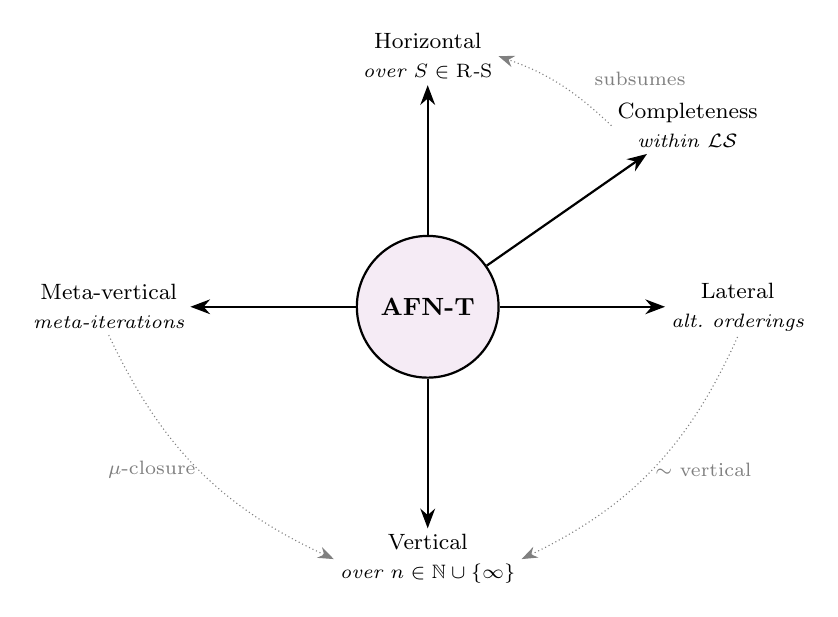
\begin{tikzpicture}[
  axis/.style={-{Stealth[length=2.5mm]}, thick},
  dep/.style={-{Stealth[length=2mm]}, thin, gray, densely dotted},
  label/.style={font=\footnotesize, align=center, inner sep=2pt},
  center/.style={draw, circle, thick, minimum size=1.8cm, align=center, font=\bfseries\small, fill=violet!8}
]
\node[center] (C) at (0,0) {AFN-T};
\node[label, above=1.9cm of C]          (H) {Horizontal \\[1pt] \scriptsize\itshape over $S \in \RS$};
\node[label, below=1.9cm of C]          (V) {Vertical \\[1pt] \scriptsize\itshape over $n \in \mathbb{N} \cup \{\infty\}$};
\node[label, left=2.1cm of C]           (M) {Meta-vertical \\[1pt] \scriptsize\itshape meta-iterations};
\node[label, right=2.1cm of C]          (L) {Lateral \\[1pt] \scriptsize\itshape alt.\ orderings};
\node[label] (K) at (3.3,2.3) {Completeness \\[1pt] \scriptsize\itshape within $\cL\cS$};
\draw[axis] (C) -- (H);
\draw[axis] (C) -- (V);
\draw[axis] (C) -- (M);
\draw[axis] (C) -- (L);
\draw[axis] (C) -- (K);
\draw[dep] (K.west) to[bend right=12] node[pos=0.35, above right=2pt and 6pt, font=\scriptsize, text=gray, inner sep=1pt] {subsumes} (H.east);
\draw[dep] (L.south) to[bend left=20] node[midway, right, font=\scriptsize, text=gray, inner sep=1pt] {$\sim$ vertical} (V.east);
\draw[dep] (M.south) to[bend right=20] node[midway, left, font=\scriptsize, text=gray, inner sep=1pt] {$\mu$-closure} (V.west);
\end{tikzpicture}
\caption{Five proposed axes of variation. The relative identity obstruction applies at each stage where its definability and categorical hypotheses have been established. The diagram does not prove that these axes exhaust all extensions or that meta-vertical iteration is a stabilized closure of finite categorical levels. Those are additional construction and scope obligations.}
\label{fig:five-axis}
\end{figure}

\begin{theorem}[Horizontal absoluteness]\label{thm:horizontal}
AFN-T (Theorem~\ref{thm:afnt-alpha}) holds for every $S \in \RS$ uniformly: there is a single proof working for all Rich-metatheories satisfying (R1)--(R5).
\end{theorem}

\begin{proof}
The proof of Theorem~\ref{thm:afnt-alpha} consists of a single application of Lemma~\ref{lem:SS-membership} (syntax--semantics bridge) together with the observation that $\id_X : X \to X$ realizes a Morita reduction violating $(\Pi_{4, S, n})$. Lemma~\ref{lem:SS-membership} uses only (R2) and (R5a) (the syntactic category exists and its objects support the pointing construction of Convention~\ref{conv:notation}); the Morita-reduction observation uses only the categorical identity morphism. No datum from $S$ beyond (R1)--(R5) is invoked. Hence the proof applies uniformly to all $S \in \RS$.
\end{proof}

\begin{theorem}[Relative vertical exclusion]\label{thm:vertical}
At every categorical level for which the syntax--semantics bridge and derived-class membership of Theorem~\ref{thm:afnt-alpha} are supplied, its candidate fails $\Pi_4$.
\end{theorem}
\begin{proof}
The identity of the candidate is an equivalence to a derived-class target, namely itself. This argument is independent of the chosen depth once those hypotheses hold. It neither constructs higher-depth syntax nor proves that an unbounded tower stabilizes.
\end{proof}

\begin{theorem}[Relative meta-vertical exclusion]\label{thm:meta-vertical}
Any meta-iteration that is actually formalized as an $S$-definable object
of the derived class $\cS_S$ fails $\Pi_4$ in that metatheory.
\end{theorem}
\begin{proof}
The identity functor on the object is an equivalence onto its image and
is one of the interpretations prohibited by $\Pi_4$. This is the same
argument as Theorem~\ref{thm:afnt-alpha}.
\end{proof}
This relative exclusion does not imply that iteration adds no structure,
that a tower stabilizes, or that all possible iterations are $S$-definable.

\begin{theorem}[Lateral absoluteness]\label{thm:lateral}
All alternative categorical orderings reduce to (or enrich) the $(\infty, n)$-hierarchy and therefore satisfy AFN-T.
\end{theorem}

\begin{proof}
Each listed ordering admits a canonical translation to $(\infty, n)$-$\Cat$ for appropriate $n$:
\begin{itemize}
\item Operads $\to$ symmetric monoidal $(\infty, 1)$-categories (Lurie HA~\cite{LurieHA} \S 5).
\item Double categories $\to$ $(\infty, 2)$-categories (Grandis).
\item Globular/cubical/opetopic $\omega$-categories $\simeq (\infty, \infty)$-categories (Ara--Maltsiniotis~\cite{AraMaltsiniotis2017}).
\item Stable $(\infty, 1)$-categories $\to (\infty, 1)$-categories via spectrification.
\item Fusion categories $\to$ finite $(\infty, 1)$-categories.
\end{itemize}
In each case, the translation preserves formal definability: objects in the alternative ordering correspond to objects in the $(\infty, n)$-hierarchy at the relevant level. Therefore, AFN-T applies uniformly across all orderings.
\end{proof}

\begin{definition}[Lawvere-scope]\label{def:law-scope}
A foundational theory $F$ belongs to the \textbf{Lawvere-scope} $\cL\cS$ if the following structural properties hold (the metatheory in which $\Syn(F)$ and $\Mod(F)$ are constructed is arbitrary but fixed throughout the four clauses):
\begin{itemize}
\item \textbf{(L1)} $F$ has a syntactic category $\Syn(F)$ --- a small category of contexts and provable substitutions.
\item \textbf{(L2)} $F$ has a semantic $2$-category $\Mod(F)$ --- the $2$-category of models.
\item \textbf{(L3)} There exists a canonical adjunction $\Syn \dashv \Mod$ (Lawvere~\cite{Lawvere1969}).
\item \textbf{(L4)} $\Mod(F)$ is realizable as an $(\infty, n)$-category for some $n$ (Grothendieck--Lurie tradition).
\end{itemize}
Membership in $\cL\cS$ is a structural property of $F$ and does not presuppose any specific R-S. In particular, every R-S $S$ is itself in $\cL\cS$ (take the tautological $\Syn = S$, $\Mod = \Mod(S)$ from (R5)), so the notion is circularity-free for the application in Theorem~\ref{thm:completeness}.
\end{definition}

\begin{theorem}[Completeness axis, conditional on Lawvere-scope]\label{thm:completeness}
Suppose $F \in \cL\cS$. Then every structural variation of $F$ reduces to one of the four axes (horizontal, vertical, meta-vertical, lateral). In particular, AFN-T is five-axis absolute within $\cL\cS$.
\end{theorem}

\begin{proof}
Let $F \in \cL\cS$. By Definition~\ref{def:law-scope}, $F$ is characterized by a quadruple:
\begin{itemize}
\item \textbf{(A) Syntactic structure $\Syn(F)$}: signature + axioms + inference rules --- the \emph{horizontal axis} (over R-S).
\item \textbf{(B) Semantic depth}: the level $n$ of $\Mod(F)$ as $(\infty, n)$-category --- the \emph{vertical axis}.
\item \textbf{(C) Meta-reflection}: iterations of G\"odel coding and reflection principles --- the \emph{meta-vertical axis}.
\item \textbf{(D) Alternative semantics}: operadic, globular, cubical, opetopic, etc.\ --- the \emph{lateral axis}.
\end{itemize}
By Definition~\ref{def:law-scope}, membership in $\cL\cS$ \emph{means} that $F$ is presented exactly by the data (L1)--(L4), i.e.\ by the quadruple (A)--(D); this is where the conditionality of the theorem resides --- within $\cL\cS$, exhaustiveness of (A)--(D) holds by definition of the scope, not as an additional claim. Thus any putative fifth axis $\eta$ is a subcomponent of one of (A)--(D). Either $\eta \subseteq$ (A), in which case AFN-T for $\eta$ reduces to horizontal absoluteness (Theorem~\ref{thm:horizontal}); $\eta \subseteq$ (B), reducing to vertical (Theorem~\ref{thm:vertical}); $\eta \subseteq$ (C), reducing to meta-vertical (Theorem~\ref{thm:meta-vertical}); or $\eta \subseteq$ (D), reducing to lateral (Theorem~\ref{thm:lateral}). There is no independent fifth axis within $\cL\cS$.
\end{proof}

\section{Three Standard Bypass Paths}\label{sec:bypass}

\begin{theorem}[Definable coherent families]\label{thm:universe}
Let $D:I\to\Cat$ be an explicitly specified small diagram, definable in
$S$, and suppose its relevant limit exists in the chosen universe and is
included among the derived constructions $\cS_S$. Then its limit belongs
to $\cS_S$ and fails $\Pi_4$ by the identity interpretation.
\end{theorem}
\begin{proof}
Membership is the stated closure assumption; the final claim is
Theorem~\ref{thm:afnt-alpha} applied to the resulting definable object.
\end{proof}
Universe-indexed endofunctors do not automatically form such a diagram:
restriction along $\cU_\ell\hookrightarrow\cU_{\ell'}$ need not send an
endofunctor of the larger universe to one of the smaller universe.
Preservation of the smaller universe and coherent transition maps must
be supplied. An individual compatible family is a section, not the
entire category of all sections.

\paragraph{Reflective consistency tower.} The second standard bypass attempts to escape AFN-T via iterated consistency assertions. One defines
\[ S_{\kappa+1} = S_\kappa + \Con(S_\kappa) \]
and hopes that the limit $S_\infty$ captures something beyond its starting point.

\begin{remark}[Consistency iterations need separate strength analysis]\label{thm:reflective}
For a specified recursively axiomatized theory $S$, adding
$\mathrm{Con}(S)$ is an arithmetical consistency extension. Its strength
is not uniformly ``exactly one inaccessible cardinal''. Transfinite
iterations require a specified notation system, limit rule and reflection
principle; none is fixed by the display $S_{\alpha+1}=S_\alpha+\mathrm{Con}(S_\alpha)$
alone. The claimed inaccessible bound and the formula adding a cardinal to
$\mathrm{Con}(S)$ are withdrawn. At each well-defined Rich stage, the
relative identity argument of AFN-T still applies; it does not measure
the stage's proof-theoretic strength or show that the tower terminates.
\end{remark}

Intensional presentations can carry data forgotten by a chosen quotient. The following section distinguishes a verified slice construction from the additional conditions needed for a nontrivial MSFS refinement. No universal intensional completion is constructed here.

I begin by defining the target $2$-category of display $2$-categories.

\begin{definition}[Display $2$-class]\label{def:display-class}
Let $\cC$ be a $2$-category with $2$-pullbacks. A \textbf{display class} $\cD \subseteq \Mor_1(\cC)$ is a class of $1$-morphisms satisfying:
\begin{itemize}
\item \textbf{(D1) Contains equivalences}: every $1$-equivalence in $\cC$ lies in $\cD$.
\item \textbf{(D2) Pullback-stable}: for $d : B \to A$ in $\cD$ and any $f : A' \to A$, the $2$-pullback $f^*d : f^*B \to A'$ exists and lies in $\cD$.
\item \textbf{(D3) Closed under composition}: if $d_1 : C \to B \in \cD$ and $d_2 : B \to A \in \cD$, then $d_2 \circ d_1 \in \cD$.
\item \textbf{(D4) Invertible-cell transport}: membership in $\cD$ is invariant under invertible $2$-cells between parallel $1$-morphisms. Chosen pullbacks are supplied with their usual coherent comparison isomorphisms. No invertibility of transport along arbitrary noninvertible $2$-cells is assumed.
\end{itemize}
\end{definition}

\begin{definition}[Display $2$-category]\label{def:display-2-cat}
A \textbf{display $2$-category} is a triple $(\cC, \cD, \iota)$ where:
\begin{itemize}
\item $\cC$ is a locally small $2$-category with $2$-pullbacks.
\item $\cD$ is a display class in $\cC$.
\item Viewing $\cD$ as the full sub-$2$-category of a specified arrow $2$-category on the chosen display arrows, $\iota:\cD\hookrightarrow\operatorname{Arr}(\cC)$ is its inclusion. The arrow-category convention is part of the chosen model.
\end{itemize}
\end{definition}

\begin{definition}[The $2$-category $\Sint$]\label{def:Sint}
For the ordinary fragment, $\Sint$ is the $2$-category of categories with pullbacks and display classes, pullback-preserving functors respecting those classes, and natural transformations. The corresponding higher target must be specified together with its level of transformations and coherence data; the list below is a typed interface for that extension, not a proof of its existence.
\begin{itemize}
\item \textbf{Objects}: display $2$-categories $(\cC, \cD, \iota)$.
\item \textbf{$1$-morphisms}: a functor $F$ preserving the chosen pullbacks up to coherent isomorphism and carrying display arrows into display arrows. Its induced arrow functor restricts to $F_\cD$, with $\operatorname{Arr}(F)\iota_1\simeq\iota_2F_\cD$. In a higher version all functors and coherence cells must be taken in the specified model.
\item \textbf{$2$-morphisms}: natural $2$-transformations $\eta : F \Rightarrow G$ whose restrictions $\eta|_\cD : F_\cD \Rightarrow G_\cD$ are coherently aligned.
\end{itemize}
\end{definition}

\begin{theorem}[A verified ordinary slice construction]\label{thm:I-existence}
Let $\mathcal B$ be a locally small ordinary category with chosen pullbacks. For $F\in\mathcal B$, set $\cC_F=\mathcal B/F$ and let $\cD_F$ be the isomorphisms in $\cC_F$. Then
\[
 \II_{\mathcal B}:\mathcal B^{\mathrm{op}}\longrightarrow\Sint,
 \qquad F\longmapsto(\mathcal B/F,\cD_F)
\]
is a contravariant pseudofunctor in the ordinary display-category fragment. Base change along an isomorphism is an equivalence.
\end{theorem}
\begin{proof}
Slices have pullbacks. Isomorphisms are stable under pullback, composition, and isomorphism of arrows. Pullback along $f:F_1\to F_2$ gives $f^*:\mathcal B/F_2\to\mathcal B/F_1$, preserving these data. The universal property of pullbacks gives coherent natural isomorphisms $\id^*\simeq\id$ and $(gf)^*\simeq f^*g^*$; uniqueness of the comparison maps gives their unit and associativity equations. An inverse base isomorphism supplies a quasi-inverse base-change functor.
\end{proof}

The result does not construct a nontrivial refinement on the full $2$-category $\cF$. The previously numbered properties are retained as the following explicit extension obligations:
\begin{enumerate}
\item[\textbf{(I-1)}] Specify the higher target and coherent action on its $2$-cells. The ordinary slice pseudofunctor does not establish this for arbitrary noninvertible cells of $\cF$.
\item[\textbf{(I-2)}] Specify how gauge transformations act. The proved construction preserves actual equivalences of its base; a chosen equivalence between model categories is not automatically such a base equivalence.
\item[\textbf{(I-3)}] To prove strict refinement of Morita, construct two specified presentations with equal Morita image and inequivalent intensional data. The former $\MLTT$/$\ETT$ example does not establish this. The relevant comparison uses intensional type theory extended by both uniqueness of identity proofs and functional extensionality~\cite{KapulkinLi2025}, not bare $\MLTT$. Moreover, normalization, decidable conversion, and decidable typing are different properties. Transporting one of them across an equivalence requires the corresponding effective syntax and rules to be preserved; a display class of arrows alone does not supply those data.
\item[\textbf{(I-4)}] Supply a classification presentation of the same variance as $\II$, a coherent comparison after forgetting display data, and a proof of the proposed localization equivalence. A contravariant $\II$ cannot be composed and identified with a covariant $\rho$ without a variance-changing construction. Yoneda does not imply $\cF/F\simeq\rho(F)$, nor does existence of a localization prove its equivalence to $\fM$.
\end{enumerate}
A higher slice construction requires the appropriate pullbacks and coherent reindexing data on the actual chosen base. These hypotheses must be verified rather than inferred from the words ``Rich-foundation''.

\begin{theorem}[Conditional slice-locality]\label{thm:slice-locality}
Let $\mathcal P$ be a fixed domain and suppose functors or pseudofunctors of compatible variance
\[
 I:\mathcal P\to\Sint,\qquad \pi:\mathcal P\to\fM,
 \qquad\tpi:\Sint\to\fM
\]
are supplied with a coherent equivalence $\tpi I\simeq\pi$. Then every $I(F)$ has base image equivalent to $\pi(F)$. If the relevant $2$-pullback exists, the intensional fibre over $m$ is
\[
 \mathrm{Int}(m):=\{m\}\mathbin{\times}^{h}_{\fM}\Sint.
\]
\end{theorem}
\begin{proof}
The first assertion evaluates the specified comparison at $F$. The second is the definition of the fibre with its required comparison-to-$m$ data. No nontriviality or fibration property follows from this definition alone.
\end{proof}
A fibre is not generally the full subcategory on objects with a given isomorphism class: its morphisms must respect the selected comparison to the base point. The existence of pullbacks in the total category does not itself prove that $\tpi$ is a fibration. Constructing the comparison in (I-4), a nontrivial fibre in (I-3), and cartesian lifting data remain separate tasks.

\begin{corollary}[Base-image constancy under the stated comparison]\label{cor:slice-level}
Under the hypotheses of Theorem~\ref{thm:slice-locality}, forgetting the intensional component of $I(F)$ returns $\pi(F)$ up to the specified equivalence.
\end{corollary}
\begin{proof}
This is the component of $\tpi I\simeq\pi$ at $F$.
\end{proof}
Constancy of a selected quotient does not prove that a refinement adds no mathematical, computational, or resource-sensitive structure.

\paragraph{Finite observational quotients.}
For an executable language, representation identity compares complete programs,
including local library bindings and output selectors. A finite observational
quotient additionally fixes the interpreter, library meanings, all evidence
consulted by admission, and the allowed continuations. Equality of complete
register traces with a separate undefined outcome gives a contextual congruence
only when all continuation and admission metadata are retained and their
updates respect that equality. Such metadata can include constant-use and
selection flags, register layout, and resource allowances. Induction on a
shared continuation proves preservation of the specified observations and
admission predicate; it does not prove equality on new inputs or equal physical
cost. A hash only indexes exact comparisons. Completed fitting witnesses,
merged representations, and unexamined search frontiers therefore require
separate reporting. Budget exhaustion is \texttt{Unknown}, distinct from
semantic undefinedness or a completed refutation. These elementary operational
distinctions do not construct the higher intensional refinement or discharge
the four obligations (I-1) through (I-4).

\subsection{The Intensional Grading}\label{sec:intensional-grading}

The former generating rule began with equivalences and used operations that preserve equivalences. It therefore cannot yield a nontrivial measure of distance from equivalence. A useful filtration needs explicitly chosen additional generators.

\begin{definition}[Grade relative to chosen generators]\label{def:display-grade}
In a specified category or $2$-category, choose a seed class $G$ of arrows saturated under the admitted invertible transports. Let $D^{(0)}=G$ and let $D^{(n+1)}$ be the invertible-transport saturation of $D^{(n)}$ together with arrows obtained by one allowed pullback or composition from arrows in $D^{(n)}$. Thus invertible comparison data have zero grade cost. Put $D=\bigcup_{n<\omega}D^{(n)}$ and
\[
 \gr_G(d)=\min\{n:d\in D^{(n)}\}.
\]
This is a grade of an arrow relative to its specified generators. It is not automatically a grade of an entire display category or of an object of an intensional fibre.
\end{definition}

\begin{proposition}[Functoriality of a generated filtration]\label{prop:grading}
Suppose a functor preserves the seed classes and each allowed generating operation, up to the admitted invertible transports. Then it preserves every stage and cannot increase grade. Composition satisfies
\[
 \gr_G(d_2d_1)\le\max(\gr_G(d_1),\gr_G(d_2))+1.
\]
If the seed class consists of all equivalences and all generating operations preserve equivalences, then every stage equals the seed class and every grade is zero.
\end{proposition}
\begin{proof}
Induct on the generating stage for the functorial assertion. Both factors of a composite are available at their maximum stage, so the composite is available at the next stage. For the last assertion, preservation of equivalences gives $D^{(n+1)}\subseteq G$, while the increasing construction always contains $G$.
\end{proof}

\begin{corollary}[Collapse of the former minimal grade]\label{cor:grade-collapse}
For the ordinary slice construction of Theorem~\ref{thm:I-existence}, the filtration generated from isomorphisms by pullbacks, composition, and isomorphism of arrows is constant at stage zero. It cannot witness a strict intensional hierarchy.
\end{corollary}
\begin{proof}
Each of the three operations preserves isomorphisms; apply Proposition~\ref{prop:grading}.
\end{proof}
An equivalence between display categories is a morphism in $\Sint$; an equivalence used as display data is an arrow inside one underlying category. These are different types. Consequently the localization class from (I-4) cannot be identified with a grade-zero class of display arrows solely by their shared name.

\begin{remark}[Remaining intensional construction]\label{rem:grading-open}
A nontrivial refinement requires generators encoding the intended syntax, evaluation, or resources; a suitable comparison relation; and verified transport of these data. Its grade is initially presentation-dependent. Invariance under equivalence, separation of Morita-equivalent presentations, strictness of successive stages, and an equivalence between the resulting localization and $\fM$ remain open. None follows from the former bare-$\MLTT$/$\ETT$ argument.
\end{remark}

\section{\texorpdfstring{$\LCls$ Meta-Classification}{Classifier Meta-Classification}}\label{sec:meta}

\subsection{\texorpdfstring{The Class $\Meta_{\mathrm{Cls}}$}{The Class Meta\_5+}}

\begin{definition}[$\LCls$ meta-structure]\label{def:meta}
An object $\mathbf{F}$ is a \textbf{$\LCls$ meta-structure} if it satisfies:
\begin{itemize}
\item \textbf{(M1) Locally small $2$-category}: $\mathbf{F}$ is a locally small $2$-category.
\item \textbf{(M2) Classification functor}: there is a $2$-functor $\Cl_{\mathbf{F}} : \mathbf{F} \to \fM$ landing in the classifying $2$-stack of Rich-foundations; we write $\fM(\mathbf{F}) := \image(\Cl_{\mathbf{F}}) \subseteq \fM$ for the sub-stack carved out by $\mathbf{F}$'s classification.
\item \textbf{(M3) Accessible reflection}: there is an accessible endofunctor $R_{\mathbf{F}} : \mathbf{F} \to \mathbf{F}$.
\item \textbf{(M4) Non-generative}: $\mathbf{F}$ does not derive the axioms of foundations $F \in \image(\Cl_{\mathbf{F}})$ from its own axioms; classification is parametric, not axiomatic.
\item \textbf{(M5) Metatheory-parametrized}: $\mathbf{F}$ is defined within some $S \in \RS$.
\end{itemize}
I denote the class of such $\mathbf{F}$ as $\Meta_{\mathrm{Cls}}$.
\end{definition}

\begin{definition}[Maximality]\label{def:maximality}
A meta-structure $\mathbf{F} \in \Meta_{\mathrm{Cls}}$ is \textbf{maximal} if additionally:
\begin{itemize}
\item \textbf{(Max-1) Full classification}: $\image(\Cl_{\mathbf{F}}) = \fM$.
\item \textbf{(Max-2) Gauge-fullness}: $\mathrm{Aut}_2(\mathbf{F})$ acts transitively on gauge classes in $\image(\Cl_{\mathbf{F}})$.
\item \textbf{(Max-3) Depth stratification}: $\mathbf{F}$ admits a \emph{depth-indexed filtration} $\mathbf{F}^{(0)} \hookrightarrow \mathbf{F}^{(1)} \hookrightarrow \cdots \hookrightarrow \mathbf{F}^{(n)} \hookrightarrow \cdots$ of accessible $2$-subcategories with $\mathbf{F} \simeq_2 \colim_{n < \omega} \mathbf{F}^{(n)}$, equipped with a \emph{depth function} $\dep : \Ob(\mathbf{F}) \to \omega$ assigning to each object the least $n$ such that the object lies in $\mathbf{F}^{(n)}$, satisfying the following \emph{predicativity condition}: for every predicate $P$ appearing in a definition by comprehension of an object $A \in \mathbf{F}^{(n)}$ (i.e., the definition has the form ``$A :=$ the object classifying $\{x : P(x)\}$''), every object $Y$ that appears as the target of a sub-expression in $P$ --- in particular every target of $R_\mathbf{F}$, $\Cl_\mathbf{F}$, or subobject-classifier evaluations --- satisfies $\dep(Y) < n$.
\item \textbf{(Max-4) Intensional completeness with separation}: a proposed maximal classifier must supply a correctly typed intensional refinement satisfying the additional requirements (I-1)--(I-4) discussed after Theorem~\ref{thm:I-existence}, together with joint separation on parallel $1$-morphisms by its extensional and intensional comparisons. This remains an axiom on a sought construction. Separation neither supplies missing morphism lifts nor proves equivalences on hom-categories.
\end{itemize}
I denote the class of maximal meta-structures as $\Meta_{\mathrm{Cls}}^{\top}$.
\end{definition}

\subsection{Meta-Categoricity: the missing lifting condition}

\begin{theorem}[Conditional comparison criterion]\label{thm:meta-cat}
Let $\mathbf F_1,\mathbf F_2$ be locally small $2$-categories over the same
metatheory. Suppose a common $2$-category $\mathbf K$ and comparison
$2$-functors $\Phi_i:\mathbf F_i\to\mathbf K$ are supplied, each essentially
surjective on objects and inducing an equivalence of categories on every
hom-category. Then $\mathbf F_1\simeq_2\mathbf F_2$.
\end{theorem}
\begin{proof}
Each $\Phi_i$ is a biequivalence by the stated object and hom conditions.
Compose $\Phi_1$ with a pseudoinverse of $\Phi_2$. The resulting comparison
depends on the supplied data; no unqualified canonical comparison is asserted.
\end{proof}

\begin{remark}[Status of the proposed maximal classifier]
Conditions (Max-1)--(Max-4) alone have not established these comparison data.
Essential surjectivity on objects does not lift morphisms: the functor from
the terminal category to $BG$, for a nontrivial group $G$, is essentially
surjective and faithful but not full. A transitive action on object classes
does not supply the missing lifts, and separation of $1$-morphisms does not
give equivalences on hom-categories. Straightening applies to an already
specified indexed category/fibration; it does not manufacture the required
universal property from an arbitrary classification functor. Constructing
the common classifier and proving the lifting and coherence conditions
remain open. Accessibility also does not recover unspecified higher cells
from a $2$-categorical comparison.
\end{remark}

\subsection{Structural Multiplicity}

\begin{theorem}[Conditional structural multiplicity]\label{thm:meta-mult}
Let $\mathbf F_1,\mathbf F_2,\mathbf F_3$ be constructed meta-structures satisfying (M1)--(M5), with classification functors $\Cl_i$ to the same base $\fM$. If their essential classification images are pairwise distinct, they are pairwise non-equivalent as classifiers over $\fM$. If each image is proper, none satisfies (Max-1).
\end{theorem}
\begin{proof}
An equivalence of classifiers over $\fM$ preserves the essential image of the classification functor. Distinct images therefore preclude such an equivalence. A proper image fails the essential-surjectivity requirement (Max-1).
\end{proof}
The programmes of Univalent Foundations, $\infty$-cosmoi, and cohesive higher topoi motivate candidates for this comparison. A programme is not itself a specified locally small $2$-category with an MSFS classification functor. Verifying (M1)--(M5), constructing those functors, and proving the claimed image distinctions are still required. In particular, being presented in one syntactic language does not exclude another presentation of the same Morita class.

\begin{corollary}[Conditional plurality at $\LCls$]\label{cor:plurality}
Under the construction and image hypotheses of Theorem~\ref{thm:meta-mult}, $\LCls$ contains multiple non-equivalent classifiers over $\fM$.
\end{corollary}

\subsection{Meta-Classification: construction and stabilization obligations}

\begin{remark}[Open meta-classification problem]\label{thm:meta-stab}
The notation $\fM^{(\mathrm{Cls})}:=\Meta_{\mathrm{Cls}}/\text{meta-gauge}$
specifies a proposed quotient, not a proof that it exists with (M1)--(M5).
One must construct its site, descent data, universe bounds and reflection.
In particular, classification of meta-structures is not automatically a
classification functor into the original stack of Rich-foundations: the
targets have different types.

An equivalence between this quotient and a second classifier requires
explicit comparison functors and invertible unit/counit. The unicity theorem
of Barwick--Schommer-Pries~\cite{BarwickSchommerPries2021} concerns models of
$(\infty,n)$-category theory for fixed finite $n$; it does not prove
idempotence of the operation of classifying foundations. This idempotence
is an open obligation, not an established result of this paper.

An unbounded tower of inaccessible universes is also an additional
metatheoretic assumption. Two inaccessible cardinals do not by themselves
provide $\kappa_1<\kappa_2<\cdots$ for arbitrary iteration depth.
\end{remark}

\begin{corollary}[Relative exclusion at any constructed stage]\label{cor:iteration-closure}
At each stage actually constructed within the chosen metatheory and meeting
the definability hypotheses of Theorem~\ref{thm:afnt-alpha}, its defining
object cannot also satisfy $\Pi_4$. This follows by applying the identity
interpretation at that stage; no stabilization assumption is needed.
\end{corollary}

\begin{remark}[Closure remains to be proved]\label{cor:meta-closure}
Closure of $\Meta_{\mathrm{Cls}}$ under meta-classification is not a
consequence of the preceding relative exclusion. It requires the separate
construction and type checks listed in Remark~\ref{thm:meta-stab}.
\end{remark}

\section{AC/OC Duality and the Dual Boundary Lemma}\label{sec:ac-oc-duality}

The Lambek--Scott adjunction $(\Syn, \Mod)$ of (R5b), assembled across $\RS$ and over $n \in \mathbb{N} \cup \{\infty\}$, induces a $(\infty, \infty)$-equivalence between the theory-centric moduli $\fM$ and the enactment-centric moduli $\fM_\cE$ (Theorem~\ref{thm:ac-oc-duality}). The dual boundary lemma $\LAbsE = \emptyset$ follows (Theorem~\ref{thm:dual-afnt}).

\begin{figure}[ht]
\centering
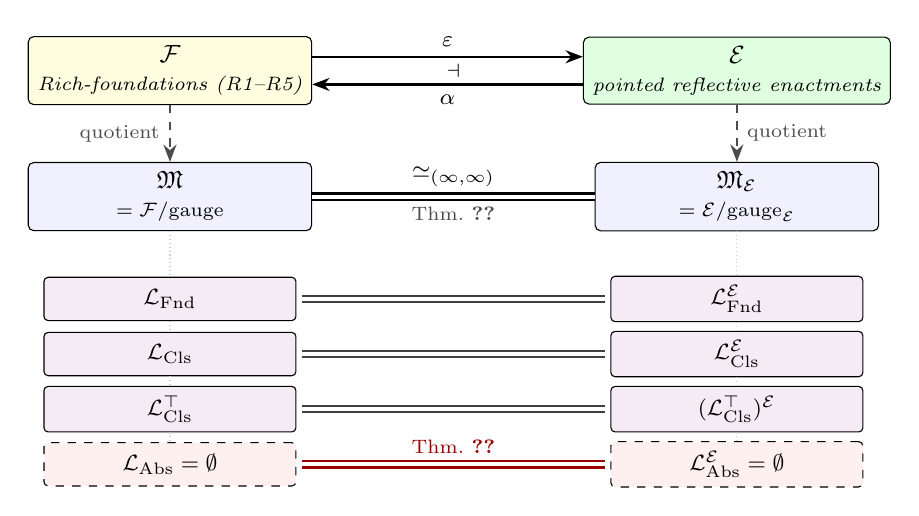
\begin{tikzpicture}[
  cat/.style={draw, rounded corners=2pt, minimum width=3.6cm, minimum height=0.85cm, align=center, font=\small},
  stack/.style={draw, rounded corners=2pt, minimum width=3.6cm, minimum height=0.85cm, align=center, font=\small, fill=blue!6},
  strat/.style={draw, rounded corners=1.5pt, minimum width=3.2cm, minimum height=0.55cm, align=center, font=\footnotesize, fill=violet!8},
  emptybox/.style={draw, dashed, rounded corners=1.5pt, minimum width=3.2cm, minimum height=0.55cm, align=center, font=\footnotesize, fill=red!6},
  func/.style={-{Stealth[length=2.2mm]}, thick},
  equiv/.style={thick, double, double distance=1.5pt},
  node distance=0.4cm
]
% Top row: 2-categories
\node[cat, fill=yellow!12] (F) at (-3.6,3.2) {$\cF$ \\[-1pt] \scriptsize\itshape Rich-foundations (R1--R5)};
\node[cat, fill=green!12] (E) at (3.6,3.2) {$\cE$ \\[-1pt] \scriptsize\itshape pointed reflective enactments};
\draw[func] ([yshift=5pt]F.east) -- node[midway, above, font=\footnotesize] {$\varepsilon$} ([yshift=5pt]E.west);
\draw[func] ([yshift=-5pt]E.west) -- node[midway, below, font=\footnotesize] {$\alpha$} ([yshift=-5pt]F.east);
\node[font=\scriptsize] at (0, 3.2) {$\dashv$};

% Middle row: moduli stacks
\node[stack] (M) at (-3.6, 1.6) {$\fM$ \\[-1pt] \scriptsize\itshape $= \cF / \mathrm{gauge}$};
\node[stack] (ME) at (3.6, 1.6) {$\fME$ \\[-1pt] \scriptsize\itshape $= \cE / \mathrm{gauge}_\cE$};
\draw[func, dashed, gray!60!black] (F) -- node[midway, left, font=\scriptsize, gray!60!black] {quotient} (M);
\draw[func, dashed, gray!60!black] (E) -- node[midway, right, font=\scriptsize, gray!60!black] {quotient} (ME);
\draw[equiv] (M.east) -- node[midway, above, font=\footnotesize] {$\simeq_{(\infty, \infty)}$} node[midway, below, font=\scriptsize, gray!60!black] {Thm.~\ref{thm:ac-oc-duality}} (ME.west);

% Bottom rows: strata correspondence
\node[strat] (L5F) at (-3.6, 0.3) {$\LFnd$};
\node[strat] (L5E) at (3.6, 0.3) {$\LFndE$};
\node[strat] (LCF) at (-3.6, -0.4) {$\LCls$};
\node[strat] (LCE) at (3.6, -0.4) {$\LClsE$};
\node[strat] (LMF) at (-3.6, -1.1) {$\LClsMax$};
\node[strat] (LME) at (3.6, -1.1) {$\LClsMaxE$};
\node[emptybox] (L6F) at (-3.6, -1.8) {$\LAbs = \emptyset$};
\node[emptybox] (L6E) at (3.6, -1.8) {$\LAbsE = \emptyset$};

\draw[equiv, gray!50!black, shorten >=2pt, shorten <=2pt] (L5F) -- (L5E);
\draw[equiv, gray!50!black, shorten >=2pt, shorten <=2pt] (LCF) -- (LCE);
\draw[equiv, gray!50!black, shorten >=2pt, shorten <=2pt] (LMF) -- (LME);
\draw[equiv, red!60!black, shorten >=2pt, shorten <=2pt] (L6F) -- node[midway, above, font=\scriptsize, red!60!black] {Thm.~\ref{thm:dual-afnt}} (L6E);

% Connect stacks to strata
\draw[gray!40, densely dotted] (M.south) -- (L5F.north);
\draw[gray!40, densely dotted] (ME.south) -- (L5E.north);
\draw[gray!40, densely dotted] (L5F.south) -- (LCF.north);
\draw[gray!40, densely dotted] (L5E.south) -- (LCE.north);
\draw[gray!40, densely dotted] (LCF.south) -- (LMF.north);
\draw[gray!40, densely dotted] (LCE.south) -- (LME.north);
\draw[gray!40, densely dotted] (LMF.south) -- (L6F.north);
\draw[gray!40, densely dotted] (LME.south) -- (L6E.north);

\end{tikzpicture}
\caption{AC/OC duality and the induced bijection of strata. At the $2$-category level (top row), the adjoint pair $\varepsilon \dashv \alpha$ (Definition~\ref{def:enactments}) relates the theory-centric $\cF$ to the enactment-centric $\cE$: $\varepsilon$ is the syntactic self-enactment section $F \mapsto (F, \Syn(F), \id, \id)$; $\alpha$ is the forgetful functor $(F, \cC, \iota, r) \mapsto F$. Passing to gauge-classes (middle row) yields an $(\infty, \infty)$-equivalence of classifying $2$-stacks $\fM \simeq \fME$ (Theorem~\ref{thm:ac-oc-duality}), via full faithfulness of $\varepsilon$ and essential surjectivity through the chosen reflector $r$. Under this equivalence the four strata correspond bijectively (bottom rows): $\LFnd \leftrightarrow \LFndE$, $\LCls \leftrightarrow \LClsE$, $\LClsMax \leftrightarrow \LClsMaxE$, and $\LAbs = \emptyset \leftrightarrow \LAbsE = \emptyset$ (Theorem~\ref{thm:dual-afnt}). The symmetry formalises the reconciliation of the object-centric and action-centric viewpoints on mathematical foundations: neither is primary; both describe the same classifying stack.}
\label{fig:ac-oc-duality}
\end{figure}

\subsection{\texorpdfstring{The $2$-Category of Rich-Enactments}{The 2-Category of Rich-Enactments}}

\begin{definition}[$2$-category of enactments $\cE$]\label{def:enactments}
The \emph{$2$-category of Rich-enactments} $\cE$ has:
\begin{itemize}
\item \textbf{Objects}: quadruples $(F, \cC, \iota, r)$, called \emph{pointed reflective enactments over $F$}, where $F \in \cF$, $\cC \in \mathbf{StrCat}_{S, n_F}$ (Definition~\ref{def:strcat}) is a $\kappa_1$-accessible $S$-model-category with an $F$-model structure, $\iota : \Syn(F) \to \cC$ is an $F$-preserving fully faithful $(\infty, n_F)$-functor onto a replete sub-$(\infty, n_F)$-category, and $r : \cC \to \Syn(F)$ is a \emph{chosen} left adjoint (reflector) to $\iota$ with unit $\eta_r : \id_\cC \Rightarrow \iota \circ r$ and counit $\varepsilon_r : r \circ \iota \Rightarrow \id_{\Syn(F)}$ satisfying the triangle identities in $\mathbf{StrCat}_{S, n_F}$. The reflector $r$ is part of the data; it is uniquely determined by $\iota$ up to unique invertible $2$-cell (Riehl--Verity~\cite{RiehlVerity2022} Prop.~2.1.11; Ad\'amek--Rosick\'y~\cite{AdamekRosicky1994} Thm.~1.26).
\item \textbf{$1$-morphisms} $(\phi, \Phi) : (F_1, \cC_1, \iota_1, r_1) \to (F_2, \cC_2, \iota_2, r_2)$: a pair consisting of a $1$-morphism $\phi : F_1 \to F_2$ in $\cF$ (faithful interpretation) and an $S$-preserving $(\infty, n)$-functor $\Phi : \cC_1 \to \cC_2$ equipped with an invertible $2$-cell $\Phi \circ \iota_1 \Rightarrow \iota_2 \circ \Syn(\phi)$;
\item \textbf{$2$-morphisms}: coherent natural transformations $(\phi, \Phi) \Rrightarrow (\phi', \Phi')$ compatible with the structure cells, i.e., pairs $(\tau, T)$ with $\tau : \phi \Rightarrow \phi'$ in $\cF$ and $T : \Phi \Rrightarrow \Phi'$ satisfying the evident pentagon with $\iota_1, \iota_2, \Syn(\tau)$.
\end{itemize}
There is a canonical forgetful $2$-functor and a canonical section:
\[
  \alpha : \cE \to \cF, \quad (F, \cC, \iota, r) \mapsto F; \qquad
  \varepsilon : \cF \to \cE, \quad F \mapsto \bigl(F,\, \Syn(F),\, \id_{\Syn(F)},\, \id_{\Syn(F)}\bigr).
\]
By construction $\alpha \circ \varepsilon = \id_\cF$ strictly. For readability I occasionally write $(F, \cC, \iota)$ for $(F, \cC, \iota, r)$ when the reflector is understood.
\end{definition}

\begin{definition}[Enactment gauge]\label{def:gauge-E}
Let $\mathcal{R}_\cE\subseteq\Mor_1(\cE)$ consist of reflection morphisms $(\tau,\Phi)$ for which $\tau$ is a gauge transformation and $r_2\Phi\iota_1$ is an equivalence. If the chosen localization exists with the required universe bounds, write
\[ \mathrm{gauge}_\cE := \text{the $2$-localization class generated by } \mathcal{R}_\cE, \qquad \fM_\cE := \cE[\mathcal{R}_\cE^{-1}] \]
A construction by Pronk's bicategory of fractions requires verification of all of its hypotheses, including the conditions on $2$-cells; closure under composition and pullbacks alone is not that verification. A zig-zag of inverted arrows yields equivalent objects, but the converse requires an additional argument in the chosen localization. The reflection $(\id_F,r):(F,\cC,\iota,r)\to\varepsilon(F)$ is a proposed arrow to invert. Its presence does not make the unit of the original reflection invertible in $\cE$.
\end{definition}

\subsection{The Enactment Syntax--Semantics Lemma}

\begin{definition}[The class $\SSE$]\label{def:SSE}
Given $S \in \RS$, the class $\SSE \subseteq \Ob \cE$ of \emph{$S$-definable pointed enactments} is the closure of the base class
\[
  \SSEbase = \bigl\{ (F', \cM, \iota_\cM, r_\cM) : \cM \models S,\ F' \in \cF,\ \iota_\cM := \ev_\cM,\ r_\cM := (\ev_\cM)^L \bigr\},
\]
where $\ev_\cM : \Syn(F') \to \cM$ is the syntax-to-semantics evaluation of (R5b) and $(\ev_\cM)^L$ is its left adjoint (Lambek--Scott), under componentwise application of the operations of Definition~\ref{def:SS}: the $F$-component by Definition~\ref{def:SS}; the $\cC$-component via the forgetful $\mathbf{StrCat}_{S, n} \to (\infty, n)\text{-}\Cat$; the $(\iota, r)$-components by functoriality of adjunctions under $S$-preserving $(\infty, n)$-functors. The sub-class $\SSEglobal \subseteq \SSE$ is the corresponding closure of $\SSEbase$ using only those operations of Definition~\ref{def:SS} defining $\cS_S^{\mathrm{global}}$ (Kan extensions, Grothendieck constructions, derived functors).
\end{definition}

\begin{lemma}[Enactment syntax--semantics lemma]\label{lem:SS-membership-E}
Let $(F, \cC, \iota, r) \in \cE$ be a pointed reflective enactment such that the quadruple is formally $S$-definable, i.e., there exist formulas $\phi_F, \psi_\cC, \chi_\iota, \chi_r$ in some $F' \in \cF$ with $F' \hookrightarrow S$ specifying $F, \cC, \iota, r$ respectively, with the triangle identities and reflectiveness of $\iota$ provable in $F'$. Then $(F, \cC, \iota, r) \in \SSEglobal$.
\end{lemma}

\begin{proof}
By hypothesis, $F$ is formally $S$-definable via $\phi_F$; Lemma~\ref{lem:SS-membership} gives $F \in \cS_S^{\mathrm{global}}$. The model-category $\cC$ is specified by $\psi_\cC$ within $F'$; as an $S$-structured $(\infty, n)$-category the underlying $(\infty, n)$-category of $\cC$ lies in $\cS_S^{\mathrm{global}}$ by the same argument applied to the $\cS_S^{\mathrm{global}}$-closure of Definition~\ref{def:SS}. The pointing $\iota$ and the reflector $r$, specified by $\chi_\iota$ and $\chi_r$ in $F'$, are morphisms between $\cS_S^{\mathrm{global}}$-objects definable in $F' \hookrightarrow S$. The adjoint pair $(\iota, r)$ is realised in $\SSEglobal$ via the following explicit construction: $\iota$ is obtained as a Kan extension (Definition~\ref{def:SS}, O1) along the inclusion $\Syn(F') \hookrightarrow \cC$ specified by $\chi_\iota$; the existence of the \emph{left} reflector $r$ (left adjoint to $\iota$ per Definition~\ref{def:enactments}) then follows from the adjoint-functor existence theorem for accessible functors between locally $\kappa_S$-presentable categories (Ad\'amek--Rosick\'y~\cite{AdamekRosicky1994}, the adjoint-functor existence theorem applied to the cocomplete-category case), with the triangle identities transported from $\chi_r$. Assembled componentwise, $(F, \cC, \iota, r) \in \SSEglobal$.
\end{proof}

\subsection{AC/OC Morita Duality}

\begin{theorem}[Conditional AC/OC comparison after localization]\label{thm:ac-oc-duality}
Work at a specified categorical level. Suppose the theory and enactment localizations $\fM$ and $\fM_\cE$ exist and the proposed functors $\varepsilon,\alpha$ descend to functors $\bar\varepsilon,\bar\alpha$ on them. Suppose there are coherent natural equivalences
\[
 \bar\alpha\bar\varepsilon\simeq\id_{\fM},\qquad
 \bar\varepsilon\bar\alpha\simeq\id_{\fM_\cE}.
\]
Then $\fM$ and $\fM_\cE$ are equivalent. Any stratum predicates and meta-operations invariant under these comparison data transfer along the equivalence.
\end{theorem}
\begin{proof}
The two displayed equivalences exhibit quasi-inverse comparison functors. A stratum or operation transfers when its defining data commute with those functors, as required by the final hypothesis.
\end{proof}
For the proposed enactments, $\alpha\varepsilon=\id$ holds before localization and the reflection morphisms suggest the second comparison. One must still prove existence and size of the localizations, descent of both functors, and naturality and coherence of the comparison on all morphisms. Inverting reflection morphisms objectwise is not a proof of all these conditions. No unbounded-depth lift follows from finite-level comparisons; Remark~\ref{thm:bergner-lurie-stab} records the missing stabilization argument.

\begin{corollary}[Conditional definitional conservativity]\label{cor:ac-oc-conservativity}
If the enactment apparatus and all its structure maps are introduced by explicit definitions whose existence and uniqueness are proved in a fixed base $B$, adjoining their names is conservative over $B$ for sentences of its original language.
\end{corollary}
\begin{proof}
Eliminate the new names by their defining formulas. Existence and uniqueness make this elimination a proof translation into $B$. Categorical equivalence alone is not this syntactic conservativity argument.
\end{proof}
Applying the corollary requires completing the construction of the enactment apparatus in $B$. No equation $\Con(\mathrm{MSFS})=\Con(\ZFC+2\text{-inacc})$ follows merely from using that metatheory. A model construction gives an upper consistency bound; a matching lower bound requires an additional interpretation.

The equivalence of Theorem~\ref{thm:ac-oc-duality} transfers the $\LAbs$ conditions of \S\ref{sec:conditions} to the enactment side. Informally, an \emph{enactment-absolute} triple $(F, \cC, \iota)$ is one whose enactment-side description simultaneously admits formal specification, admits no non-trivial coordination with other enactments in the $S$-definable class, and is maximally receptive (every other enactment factors through it).

\begin{definition}[$\LAbsE$ conditions]\label{def:level6-cE}
Given $S \in \RS$ and $n \in \mathbb{N} \cup \{\infty\}$, a pointed reflective enactment $(F, \cC, \iota, r) \in \cE$ is \textbf{enactment-absolute} if it satisfies the triple:
\begin{itemize}
\item[$(\tilde{F}_S)$] \emph{Enactment-definability}: the quadruple $(F, \cC, \iota, r)$ is formally $S$-definable in the sense of Lemma~\ref{lem:SS-membership-E}, i.e., specified by formulas $(\phi_F, \psi_\cC, \chi_\iota, \chi_r)$ in some $F' \in \cF$ with $F' \hookrightarrow S$ (this refines $(F_S)$ by additionally specifying the model-category presentation, the pointing, and the reflector).
\item[$(\tilde{\Pi}_{4, S, n})$] \emph{Non-coordination}: there is no $1$-morphism $(\phi, \Phi) : (F, \cC, \iota, r) \to (F', \cC', \iota', r')$ in $\cE$ with target quadruple in $\SSE$ (Definition~\ref{def:SSE}) such that $\Phi$ is an $(\infty, n)$-equivalence onto its image.
\item[$(\tilde{\Pi}_{3\text{-max}, S, n})$] \emph{Maximal receptivity}: for every enactment $(F', \cC', \iota', r') \in \cE$ there exists a $1$-morphism $(\phi, \Phi) : (F', \cC', \iota', r') \to (F, \cC, \iota, r)$ realizing a Morita reduction at the $(\infty, n)$-level.
\end{itemize}
The \emph{$\LAbsE$ stratum} is the class of $\mathrm{gauge}_\cE$-equivalence classes in $\fM_\cE$ with an enactment-absolute representative.
\end{definition}

\subsection{Dual Boundary Lemma}

\begin{theorem}[Dual Boundary Lemma; Dual-AFN-T $(\alpha)$-part]\label{thm:dual-afnt}
For every Rich-metatheory $S \in \RS$ and every categorical level $n \in \mathbb{N} \cup \{\infty\}$, no pointed reflective enactment $(F, \cC, \iota, r) \in \cE$ satisfies the $\LAbsE$ triple $(\tilde{F}_S) \wedge (\tilde{\Pi}_{4, S, n}) \wedge (\tilde{\Pi}_{3\text{-max}, S, n})$. Already the sub-pair $(\tilde{F}_S) \wedge (\tilde{\Pi}_{4, S, n})$ is structurally self-contradictory.
\end{theorem}

\begin{proof}
Suppose $(F, \cC, \iota, r) \in \cE$ satisfies $(\tilde{F}_S) \wedge (\tilde{\Pi}_{4, S, n})$. By Lemma~\ref{lem:SS-membership-E}, $(F, \cC, \iota, r) \in \SSEglobal \subseteq \SSE$. The identity $1$-morphism $(\id_F, \id_\cC)$ has $\Phi = \id_\cC$ an $(\infty, n)$-equivalence onto its image, with target in $\SSE$. This coordination is forbidden by $(\tilde{\Pi}_{4, S, n})$. Contradiction. Hence $\LAbsE = \emptyset$.
\end{proof}

\begin{corollary}[$\LAbsE$ emptiness]\label{cor:level6-empty-cE}
$\LAbsE = \emptyset$.
\end{corollary}

\begin{theorem}[Conditional transfer of relative axes]\label{thm:dual-five-axis}
Whenever an axis comparison preserves the hypotheses of the relative boundary lemma and satisfies the descent and coherence conditions of Theorem~\ref{thm:ac-oc-duality}, the corresponding relative exclusion transfers to the enactment presentation.
\end{theorem}
\begin{proof}
Translate a proposed witness along the assumed comparison and apply the boundary lemma in the target presentation. Preservation of its predicates is a hypothesis of this transfer, not a consequence of the name of the axis.
\end{proof}
This does not provide a general exclusion for universe changes, reflection principles, or arbitrary operational refinements. A closed symmetric monoidal category need not be cartesian closed and does not automatically support the cartesian Lawvere diagonal.

\section{Placement in the No-Go Series}\label{sec:series}

AFN-T occupies a position in the structural series of foundational no-go theorems. All such results instantiate a single categorical schema: \emph{a system sufficiently expressive to formulate a candidate maximal object is unable to contain that object without contradiction}, realized through a self-referential embedding that turns the purported maximal object into an element of the very class it was supposed to transcend. Each specializes the schema through a distinct maximality aspect and diagonal step:

\begin{center}
\begin{tabular}{@{}l l p{3.2cm} p{5.7cm}@{}}
\toprule
Theorem & Year & Maximality aspect & Diagonal step \\ \midrule
Cantor~\cite{Cantor1891} & 1891 & cardinal & $x \notin f(x)$ for $f : X \to \cP(X)$ \\
Russell~\cite{Russell1903} & 1903 & comprehension & $R = \{x : x \notin x\}$, $R \in R \iff R \notin R$ \\
G\"odel (I, II)~\cite{Godel1931} & 1931 & completeness / consistency & $G = $ ``$G$ is not provable'' \\
Tarski~\cite{Tarski1936} & 1936 & semantic truth & ``this sentence is not true'' \\
Lawvere FP~\cite{Lawvere1969} & 1969 & categorical fixed-point & cartesian-closed + weakly surjective $\Rightarrow$ every $f$ has a fixed point \\
Ernst~\cite{Ernst2015} & 2015 & unlimited category theory & Lawvere diagonal at $n = 1$ under Feferman (R1)--(R3) \\
AFN-T & --- & foundational (definable + non-reducible + generative) & syntax--semantics bridge: $(F_S) \Rightarrow X \in \cS_S^{\mathrm{global}}$ via Lemma~\ref{lem:SS-membership}, contradicting $(\Pi_4)$ by $\id_X$ (Theorem~\ref{thm:afnt-alpha}) \\
Dual-AFN-T & --- & enactment-absolute (definable + non-coordination + receptive) & identity enactment $(\id_F, \id_\cC)$ with target in $\SSE$ (Lemma~\ref{lem:SS-membership-E}) contradicts $(\tilde{\Pi}_4)$ (Theorem~\ref{thm:dual-afnt}); equivalently via $\alpha$ + AFN-T \\
\bottomrule
\end{tabular}
\end{center}

\subsection{Subsumption}

\begin{theorem}[Subsumption via specialization (framework-level)]\label{thm:subsumption}
For each classical no-go theorem $T$ below, there exists a triple $(S_T, n_T, X_T)$ with $S_T \in \RS$, $n_T \in \mathbb{N} \cup \{\infty\}$, and $X_T$ the purported maximal object of $T$, such that (i) $X_T \models (F_{S_T})$; (ii) $X_T$ under the hypothesis of $T$ would satisfy $(\Pi_{4, S_T, n_T})$; (iii) Theorem~\ref{thm:afnt-alpha} applied at $(S_T, n_T)$ yields a structural contradiction with the existence of $X_T$ as $\LAbs$-candidate. The theorem provides the \emph{framework} in which each classical no-go inhabits; the row-specific diagonals (Cantor's $|X|<|\cP(X)|$, Russell's $R \in R \leftrightarrow R \notin R$, etc.)\ are independent classical proofs that refine the abstract $\id_{X_T}$-template into the specific witness used by $T$, and are not derived from AFN-T~$\alpha$ alone.
\begin{center}\footnotesize
\begin{tabular}{@{}lllcl@{}}
\toprule
$T$ & $S_T$ & $X_T$ & $n_T$ & $(F_{S_T})$-witness \\ \midrule
Cantor~\cite{Cantor1891} & $\ZFC$ & $\cP : \mathbf{Set} \to \mathbf{Set}$ universal & $1$ & $\phi_{\cP}(X,Y) \equiv Y = \cP(X)$ \\
Russell~\cite{Russell1903} & $\ZFC$ & set of $\{x : x \notin x\}$ & $1$ & $\phi_R(x) \equiv x \notin x$ \\
G\"odel I~\cite{Godel1931} & $\mathsf{PA}$ & $G$ (unprovable sentence) & $1$ & $\phi_G \equiv \neg \mathrm{Prov}(\ulcorner G \urcorner)$ \\
G\"odel II~\cite{Godel1931} & $\mathsf{PA}$ & internal $\mathrm{Con}(\mathsf{PA})$-proof & $1$ & $\phi_{\mathrm{Con}}$ via $\mathrm{Prov}$ \\
Tarski~\cite{Tarski1936} & $\mathsf{PA}$ & arithmetical truth predicate & $1$ & $T(\phi) \equiv \phi$ \\
Lawvere FP~\cite{Lawvere1969} & CCC ext.\ of $\ZFC$ & w.\ surj.\ $X$, $f:X \to X^X$ & $1$ & $\phi_X$ in CCC-syntax \\
Ernst~\cite{Ernst2015} & Feferman (R1)--(R3) & UCT object & $1$ & Feferman unlim.\ schema \\
\bottomrule
\end{tabular}
\end{center}
In each row, AFN-T at $(S_T, n_T)$ yields $\LAbs(S_T, n_T) = \emptyset$ at the row's maximality aspect; the classical diagonal of $T$ is the specific witness refinement establishing $T$ within the framework.
\end{theorem}

\begin{proof}
Each row's $X_T$ is $S_T$-definable by the listed formula (i), so $X_T \in \cS_{S_T}^{\mathrm{global}}$ by Lemma~\ref{lem:SS-membership}. $\id_{X_T} : X_T \to X_T$ violates $(\Pi_{4, S_T, n_T})$ per Theorem~\ref{thm:afnt-alpha}, so $X_T \notin \LAbs$. The row-specific diagonal reconstructs: Cantor by $|X| < |\cP(X)|$ refining $\id_{\cP}$; Russell by $R \in R \leftrightarrow R \notin R$ refining $\id_R$; G\"odel by $G$-sentence $\leftrightarrow \neg\mathrm{Prov}(\ulcorner G \urcorner)$; Tarski's liar; Lawvere's fixed-point formula $f(x_0) = x_0$ via $\lambda x. f(x)(x)$; Ernst by Feferman unlimited-axiom schema. Each refinement specializes the universal $\id_{X_T}$ template of Theorem~\ref{thm:afnt-alpha} to the row-specific formal witness.
\end{proof}

\section{Consequences and Open Questions}\label{sec:consequences}

\subsection{Consequences for Foundational Programmes}

AFN-T imposes a uniform structural bound on every current foundational programme: each inhabits $\LFnd$, or $\LCls$ (possibly with membership in the maximal sub-class $\LClsMax \subseteq \LCls$), with $\LAbs$ empty. Specifically:
\begin{itemize}\setlength{\itemsep}{1pt}
\item \textbf{Univalent Foundations}, higher topoi, and cohesive frameworks motivate candidate classifiers. Their exact MSFS membership and classification images require the construction and verification specified in Theorem~\ref{thm:meta-mult}.
\item \textbf{Higher topos theory} supplies semantic structures; an MSFS classifying functor is further data, and no programme-level maximality verdict is inferred without it.
\item \textbf{Condensed mathematics}, perfectoid geometry, and $\infty$-cosmoi remain mathematical frameworks whose utility and potential extensions are not bounded by the relative $\Pi_4$ exclusion.
\item \textbf{Proof assistants} (Coq, Lean, Agda) implement $\LFnd$ foundations ($\CIC$, $\CIC + \mathrm{Univalence}$, $\MLTT$); the plurality of such systems is the plurality of $\LFnd$.
\item \textbf{Categorical logic}: fixed-depth comparisons can organize specified foundational presentations. No upper bound on further classifier structure follows from the finite-$n$ unicity theorem.
\end{itemize}

\paragraph{Diagnostic for a specified candidate.} First specify the formal object, its metatheory, and the relevant interpretation relation. If the candidate belongs to the derived class $\cS_S$, its identity violates $\Pi_4$ as defined here. This is the relative obstruction of AFN-T. Assigning particular research programmes to $\LCls\setminus\LClsMax$ additionally requires the classifier constructions and essential-image checks of Theorem~\ref{thm:meta-mult}; absence of a syntactic presentation in one language is not proof of absence of a Morita-equivalent presentation.

\subsection{Open Questions}

\paragraph{(Q1) Existence and comparison of maximal meta-frameworks.} Construct a concrete classifier satisfying (Max-1)--(Max-4) in a specified metatheory. Separately, construct a common comparison target and prove essential surjectivity and equivalences on all hom-categories, as required by Theorem~\ref{thm:meta-cat}. Non-emptiness alone does not imply categoricity. The four maximality clauses are distinct requirements; their logical independence has not been proved.

\paragraph{(Q2) Completeness of the meta-framework list.} How complete is the list $\{\mathbf{F}_{\mathrm{univalent}},\allowbreak \mathbf{F}_{\mathrm{cosmoi}},\allowbreak \mathbf{F}_{\mathrm{cohesive}},\allowbreak \mathbf{F}_{\mathrm{HA}},\allowbreak \mathbf{F}_{\mathrm{synthetic}}\}$ of currently identified $\LCls$ meta-structures ($\mathbf{F}_{\mathrm{HA}}$ denotes Lurie's Higher Algebra programme~\cite{LurieHA})? Are there further natural meta-frameworks?

\paragraph{(Q3) Exhaustiveness of bypass paths.} Theorems~\ref{thm:universe} and~\ref{thm:reflective} apply to explicitly definable constructions under their closure assumptions. They do not rule out all universe changes, reflection principles, or non-classical foundations. The classifier, intensional, and paraconsistent comparisons need their own construction and preservation proofs. No formal exhaustiveness result for arbitrary extensions is established.

\paragraph{(Q4) Consistency-strength minimality.} Determine the base needed for each completed construction separately. The proposed meta-stabilization in Remark~\ref{thm:meta-stab} remains open, so neither its sufficiency under two inaccessibles nor a minimal consistency strength has been established.

\paragraph{(Q5) Sub-stack of weak Rich-metatheories.} Do bounded-arithmetic theories ($\mathsf{I\Delta_0}$, $\mathsf{S}_2^i$) satisfying (R2)--(R5) and a restricted (R1) form a separate stratum $\LFnd^{\mathrm{weak}} \subset \LFnd$, or are they Morita-dense in $\LFnd$ via reverse mathematics~\cite{Simpson2009}?

\appendix

\section{Categorical Preliminaries}\label{app:categorical}

I collect here the categorical tools and standard theorems invoked in the proofs above.

\subsection{\texorpdfstring{$2$-Categories}{2-Categories}}

A \textbf{$2$-category} $\cC$ consists of:
\begin{itemize}
\item A class of objects $\Ob(\cC)$.
\item For each pair $A, B \in \Ob(\cC)$, a small category $\Hom_\cC(A, B)$ of $1$-morphisms and $2$-morphisms.
\item Composition functors and identity $1$-morphisms satisfying standard $2$-categorical coherence.
\end{itemize}

A $2$-category is \textbf{locally small} if each $\Hom_\cC(A, B)$ is a small category. All $2$-categories in this paper are locally small unless stated otherwise.

Reference: Kelly~\cite{Kelly1982} for enriched and $2$-categorical foundations; B\'enabou~\cite{Benabou1967} for bicategories.

\subsection{\texorpdfstring{$(\infty, n)$-Categories}{(infinity,n)-Categories}}

An $(\infty, n)$-category is a generalization of category theory where:
\begin{itemize}
\item Morphisms have $k$-morphisms for $k \leq n$.
\item $k$-morphisms for $k > n$ are all invertible (equivalences).
\end{itemize}

Models include: quasi-categories, Segal $n$-categories, complete Segal spaces, $\Theta_n$-spaces. Equivalence of these models is established by Ara--Maltsiniotis~\cite{AraMaltsiniotis2017}.

No unbounded-depth stabilization follows from these finite-depth comparisons. In particular, an expression such as $(\infty,\infty+1)$ requires a chosen meaning, and an equivalence with $(\infty,\infty)$ cannot be obtained merely by applying fixed-finite-$n$ unicity repeatedly; see Remark~\ref{thm:bergner-lurie-stab}.

Reference: Lurie HTT~\cite{LurieHTT} for $(\infty, 1)$-categories; Riehl--Verity~\cite{RiehlVerity2022} for synthetic $(\infty, 1)$-category theory.

\subsection{Accessible Functors}

A functor $F : \cC \to \cD$ between locally small categories is \textbf{$\lambda$-accessible} (for a regular cardinal $\lambda$) if $F$ preserves $\lambda$-filtered colimits.

A category $\cC$ is \textbf{locally $\lambda$-presentable} if it is cocomplete and has a small dense subcategory of $\lambda$-presentable objects.

Reference: Ad\'amek--Rosick\'y~\cite{AdamekRosicky1994} for accessibility theory.

\begin{lemma}[Lair--Makkai--Par\'e representation]\label{lem:lair}
Every accessible category is $2$-categorically equivalent to the $2$-category of models of a small sketch; equivalently, to the $2$-category of models of an accessible $2$-theory.
\end{lemma}

\noindent\emph{Reference for the proof.} Lair~\cite{Lair1981} ($1$-categorical sketches, original French source); Makkai--Par\'e~\cite{MakkaiPare1989} Chapter~3 (systematic development, including the $2$-categorical sketch/theory correspondence); Ad\'amek--Rosick\'y~\cite{AdamekRosicky1994} Chapter~2 (accessibility-theoretic treatment).  The lemma is used in this paper only through these references.

\subsection{Display Map Categories}

\begin{definition}[Display map category, $1$-categorical version]\label{def:display-1cat}
A \textbf{display map category} is a pair $(\cC, \cD)$ where $\cC$ is a category with pullbacks and $\cD \subseteq \Mor(\cC)$ is a class of morphisms stable under pullback and containing isomorphisms.
\end{definition}

Jacobs~\cite{Jacobs1999} establishes that display map categories provide categorical semantics for intensional type theories, with display morphisms corresponding to dependent type families.

Gambino--Garner~\cite{GambinoGarner2008} extends this to the $2$-categorical setting, yielding Definitions~\ref{def:display-class} and~\ref{def:display-2-cat}.

\subsection{Bicategory of Fractions}

\begin{lemma}[Pronk's bicategory of fractions]\label{lem:pronk}
Given a $2$-category $\cC$ and a class $\mathcal{W}$ of $1$-morphisms satisfying the Bousfield--Pronk calculus-of-fractions conditions (BF1)--(BF5), the $2$-localization $\cC[\mathcal{W}^{-1}]$ exists as a bicategory of fractions.
\end{lemma}

Reference: Pronk~\cite{Pronk1996}.

The conditions (BF1)--(BF5) are:
\begin{itemize}
\item[\textbf{(BF1)}] Contains identities.
\item[\textbf{(BF2)}] Closed under composition.
\item[\textbf{(BF3)}] $2$-pullback stable.
\item[\textbf{(BF4)}] $2$-right-filtered (any morphism can be extended).
\item[\textbf{(BF5)}] $\mathcal{W}$-saturation: contains all $2$-equivalences.
\end{itemize}

\subsection{Lawvere Fixed-Point Theorem}

\begin{lemma}[Lawvere fixed-point, $2$-categorical]\label{lem:lawvere-2}
In a $2$-cartesian closed category $\cC$ with a weakly point-surjective $1$-morphism $e : A \to Y^A$, every $f : Y \to Y$ has a fixed point: there exists $y_0 : 1 \to Y$ with $f \circ y_0 = y_0$ up to coherent $2$-equivalence.
\end{lemma}

Reference: Lawvere~\cite{Lawvere1969}; Yanofsky~\cite{Yanofsky2003} for $2$-categorical formulation.

\begin{lemma}[Conditional Lawvere result in a homotopy category]\label{lem:lawvere-inf}
Let a chosen higher-categorical model have a cartesian closed homotopy category $h\cC$. Suppose $e:A\to Y^A$ is weakly point-surjective in $h\cC$. Then every endomorphism $f:Y\to Y$ has a fixed global point in $h\cC$.
\end{lemma}
\begin{proof}
Apply the ordinary categorical diagonal argument in $h\cC$: represent the map $a\mapsto f(e(a)(a))$ by a point $a_0$ and evaluate at $a_0$. The resulting point $y_0=e(a_0)(a_0)$ satisfies $f(y_0)=y_0$ in $h\cC$.
\end{proof}
This conclusion is an equality in the homotopy category. A stronger coherent higher fixed-point structure requires a definition and further data. Finite-depth unicity does not construct a compatible family of fixed points or its limit.

\subsection{Whitehead-Type Criterion}

\begin{lemma}[Conditional reconstruction from a tower]\label{lem:whitehead}
Suppose the specified model reconstructs $\cC_i$ as the limit of a tower
$\cC_i^{(n)}$, and a functor $\Phi$ is the limit of a compatible family
of equivalences $\Phi_n:\cC_1^{(n)}\to\cC_2^{(n)}$. Then $\Phi$ is an
equivalence.
\end{lemma}
\begin{proof}
Limits preserve equivalences of diagrams. The reconstruction and
compatibility hypotheses supply the indicated diagrams and their limits.
\end{proof}
Accessibility alone does not establish reconstruction from truncations.
Applications must verify this additional completeness property in their
chosen higher-categorical model.

\subsection{The missing enrichment comparison}

\begin{remark}[No unbounded stabilization theorem supplied]\label{thm:bergner-lurie-stab}
Writing $\colim_{n<\omega}(\infty,n)\text{-}\Cat$ does not prove that
enrichment commutes with that colimit. Even when each hom-object has some
finite depth, a family of hom-objects can have unbounded depths and need
not come from any single finite stage. A cofinal shift of a diagram leaves
its colimit unchanged; it does not identify enrichment of the colimit
with the shifted diagram's colimit.

Barwick--Schommer-Pries~\cite{BarwickSchommerPries2021} establish unicity
for fixed finite $n$, with space of theories $B(\mathbb Z/2)^n$.
Their result supplies neither this interchange nor an equivalence between
successive moduli spaces of foundations. The former ``Bergner--Lurie
stabilization theorem'' and its proof by this interchange are withdrawn.
An unbounded-depth model and its comparison maps must first be specified.
\end{remark}

\section{Paraconsistent Extension}\label{app:paraconsistent}

AFN-T as stated (Theorem~\ref{thm:afnt-alpha}) applies to classical Rich-metatheories. This appendix extends the result to paraconsistent Rich-metatheories \emph{with extractable classical kernel} --- the class of paraconsistent logics in which every theorem admits a classical-inference witness. The extension does \emph{not} cover strongly-dialetheic theories (see below).

\subsection{Paraconsistent R-S}

\begin{definition}[Paraconsistent R-S with extractable classical kernel]\label{def:paraconsistent-rs}
A theory $S'$ is a \textbf{paraconsistent Rich-metatheory with extractable classical kernel} if it satisfies the classical conditions (R1')--(R5') analogous to (R1)--(R5), together with:
\begin{itemize}
\item \textbf{(Explosion-min)}: $\bot \not\vdash \phi$ for every formula $\phi$ (contradictions do not entail everything).
\item \textbf{(Strong-neg)}: there exists a negation $\sim$ such that $(p \wedge \sim p) \vdash_\sim \bot$ (a specific contradiction principle, though not full explosion).
\item \textbf{(Classical-kernel extractability)}: an explicitly specified classical fragment $S^*$ is consistent and belongs to $\RS$. Preservation of candidate definitions, interpretations, and boundary predicates under a translation from $S'$ is additional data, as required by Theorem~\ref{thm:paraconsistent-afnt}. No largest such fragment is asserted to exist automatically.
\end{itemize}
\end{definition}

\subsection{Paraconsistent AFN-T}

\begin{theorem}[Conditional transfer to a paraconsistent presentation]\label{thm:paraconsistent-afnt}
Suppose a specified classical Rich-metatheory $S^*$ and a translation from $S'$ to $S^*$ are given. Assume that this translation sends every candidate satisfying all three $\LAbs$ conditions in $S'$ to a candidate satisfying all three conditions in $S^*$. Then no such candidate exists in $S'$.
\end{theorem}
\begin{proof}[Proof (sketch)]
A candidate in $S'$ would translate to a candidate in $S^*$, contradicting Theorem~\ref{thm:afnt-alpha} there.
\end{proof}
Neither a strong negation nor the name ``classical kernel'' constructs this translation. Consistency and Rich-membership of a kernel, functoriality of the translation, and preservation of $\Pi_4$ in particular remain obligations. Removing negation symbols is not a semantics-preserving translation. The former appeal to details in an unspecified companion note does not discharge these obligations.

\section{Verum Verification Ledger}\label{app:verification-ledger}

The companion \textbf{Verum MSFS Corpus} is reported at \url{https://github.com/gst-st/msfs}. Its proof coverage must be checked against the exact statements and assumptions of this revision. The present revision does not assert that every theorem, definition, or open construction has a machine-checked proof. In particular, the newly explicit lifting and stabilization obligations cannot be counted as discharged by a previously matching label.

A verification report must identify the corpus and kernel revisions, the translated statement for each item, every admitted axiom or framework assumption, and a successful replay command. A marker of the form \texttt{@framework(name, "citation")} records a dependency; it does not prove the cited theorem or its applicability. Definitional conservativity, consistency strength, and correspondence between a formal encoding and the prose statement remain distinct obligations. No fresh replay of the external corpus is certified here.

\section*{Acknowledgments and disclosures}

The author thanks the mathematical community for the foundational results of Cantor, Russell, G\"odel, Tarski, Lawvere, Lambek--Scott, Ad\'amek--Rosick\'y, Makkai--Par\'e, Jacobs, Pronk, Lurie, Riehl--Verity, Voevodsky, Schreiber, and Clausen--Scholze, on which this synthesis rests. Max Sereda is the sole author; conceptualisation, formal analysis, proofs, and writing are entirely the author's responsibility. The work was conducted independently; the author declares no competing interests and no external funding. No data were generated or analysed; the full LaTeX source is archived with the preprint deposit.

\begin{thebibliography}{99}

\bibitem{Aczel1988}
P.~Aczel,
\newblock \emph{Non-Well-Founded Sets},
\newblock CSLI Lecture Notes 14, Stanford, 1988.

\bibitem{AdamekRosicky1994}
J.~Ad\'amek and J.~Rosick\'y,
\newblock \emph{Locally Presentable and Accessible Categories},
\newblock London Mathematical Society Lecture Notes 189, Cambridge University Press, 1994.

\bibitem{AraMaltsiniotis2017}
D.~Ara and G.~Maltsiniotis,
\newblock \emph{Homotopy comparison of cubical and globular models of weak $\omega$-categories},
\newblock Preprint, 2017.

\bibitem{AwodeyWarren2009}
S.~Awodey and M.~Warren,
\newblock Homotopy theoretic models of identity types,
\newblock \emph{Mathematical Proceedings of the Cambridge Philosophical Society} 146 (2009), 45--55.

\bibitem{Bakovic2010}
I.~Bakovi\'c,
\newblock \emph{Fibrations of bicategories},
\newblock Preprint, 2010.

\bibitem{Rezk2010}
C.~Rezk,
\newblock A Cartesian presentation of weak $n$-categories,
\newblock \emph{Geometry \& Topology} 14 (2010), no.~1, 521--571; arXiv:0901.3602.

\bibitem{Benabou1967}
J.~B\'enabou,
\newblock Introduction to bicategories,
\newblock in \emph{Reports of the Midwest Category Seminar}, Lecture Notes in Mathematics 47, Springer, 1967, pp.~1--77.

\bibitem{BergnerRezk2013}
J.E.~Bergner and C.~Rezk,
\newblock Comparison of models for $(\infty, n)$-categories, I,
\newblock \emph{Geometry \& Topology} 17 (2013), no.~4, 2163--2202.

\bibitem{BarwickSchommerPries2021}
C.~Barwick and C.~Schommer-Pries,
\newblock On the unicity of the theory of higher categories,
\newblock \emph{Journal of the American Mathematical Society} 34 (2021), 1011--1058; arXiv:1112.0040.

\bibitem{Cantor1891}
G.~Cantor,
\newblock \"Uber eine elementare Frage der Mannigfaltigkeitslehre,
\newblock \emph{Jahresbericht der Deutschen Mathematiker-Vereinigung} 1 (1891), 75--78.

\bibitem{ClausenScholze2019}
D.~Clausen and P.~Scholze,
\newblock \emph{Lectures on Condensed Mathematics},
\newblock Lecture notes, University of Bonn, 2019,
\newblock \url{https://www.math.uni-bonn.de/people/scholze/Condensed.pdf}.

\bibitem{Ernst2015}
M.~Ernst,
\newblock The prospects of unlimited category theory: doing what remains to be done,
\newblock \emph{Review of Symbolic Logic} 8 (2015), no.~2, 306--327.

\bibitem{Feferman1964}
S.~Feferman,
\newblock Systems of predicative analysis,
\newblock \emph{Journal of Symbolic Logic} 29 (1964), no.~1, 1--30.

\bibitem{Shulman2019}
M.A.~Shulman,
\newblock All $(\infty, 1)$-toposes have strict univalent universes,
\newblock preprint, 2019; arXiv:1904.07004.

\bibitem{GagnaHarpazLanari2021}
A.~Gagna, Y.~Harpaz, and E.~Lanari,
\newblock Gray tensor products and lax functors of $(\infty, 2)$-categories,
\newblock \emph{Advances in Mathematics} 391 (2021), 107986; arXiv:2002.06055.

\bibitem{GambinoGarner2008}
N.~Gambino and R.~Garner,
\newblock The identity type weak factorisation system,
\newblock \emph{Theoretical Computer Science} 409 (2008), 94--109.

\bibitem{Godel1931}
K.~G\"odel,
\newblock \"Uber formal unentscheidbare S\"atze der Principia Mathematica und verwandter Systeme I,
\newblock \emph{Monatshefte f\"ur Mathematik und Physik} 38 (1931), 173--198.

\bibitem{Hermida1999}
C.~Hermida,
\newblock Some properties of Fib as a fibred $2$-category,
\newblock \emph{Journal of Pure and Applied Algebra} 134 (1999), 83--109.

\bibitem{KapulkinLi2025}
C.~Kapulkin and Y.~Li,
\newblock Extensional concepts in intensional type theory, revisited,
\newblock \emph{Theoretical Computer Science} 1029 (2025), 115051; arXiv:2310.05706.

\bibitem{Hofmann1995}
M.~Hofmann,
\newblock \emph{Extensional concepts in intensional type theory},
\newblock PhD thesis, University of Edinburgh, 1995.

\bibitem{Hyland1982}
J.M.E.~Hyland,
\newblock The effective topos,
\newblock in \emph{The L.E.J. Brouwer Centenary Symposium}, Studies in Logic and the Foundations of Mathematics 110, North-Holland, 1982, pp.~165--216.

\bibitem{Jacobs1999}
B.~Jacobs,
\newblock \emph{Categorical Logic and Type Theory},
\newblock Studies in Logic 141, Elsevier, 1999.

\bibitem{Bishop1967}
E.~Bishop,
\newblock \emph{Foundations of Constructive Analysis},
\newblock McGraw-Hill, 1967.

\bibitem{BridgesVita2006}
D.S.~Bridges and L.S.~Vita,
\newblock \emph{Techniques of Constructive Analysis},
\newblock Universitext, Springer, 2006.

\bibitem{Buss1986}
S.R.~Buss,
\newblock \emph{Bounded Arithmetic},
\newblock Bibliopolis, Naples, 1986.

\bibitem{EseninVolpin1961}
A.S.~Esenin-Volpin,
\newblock Le programme ultra-intuitionniste des fondements des math\'ematiques,
\newblock in: \emph{Infinitistic Methods}, Pergamon Press / PWN, Warsaw, 1961, pp.~201--223.

\bibitem{EseninVolpin1970}
A.S.~Esenin-Volpin,
\newblock The ultra-intuitionistic criticism and the antitraditional program for foundations of mathematics,
\newblock in: A.~Kino, J.~Myhill, R.E.~Vesley (eds.), \emph{Intuitionism and Proof Theory}, North-Holland, 1970, pp.~3--45.

\bibitem{MarkovNagornyj1988}
A.A.~Markov and N.M.~Nagornyj,
\newblock \emph{The Theory of Algorithms},
\newblock Mathematics and its Applications (Soviet Series), Kluwer, 1988 (English translation of Nauka, Moscow, 1984).

\bibitem{Simpson2009}
S.G.~Simpson,
\newblock \emph{Subsystems of Second Order Arithmetic},
\newblock 2nd ed., Cambridge University Press, 2009.

\bibitem{LambekScott1986}
J.~Lambek and P.J.~Scott,
\newblock \emph{Introduction to Higher-Order Categorical Logic},
\newblock Cambridge Studies in Advanced Mathematics 7, Cambridge University Press, 1986.

\bibitem{KapulkinLumsdaine2021}
K.~Kapulkin and P.L.~Lumsdaine,
\newblock The simplicial model of univalent foundations (after Voevodsky),
\newblock \emph{Journal of the European Mathematical Society} 23 (2021), no.~6, 2071--2126; arXiv:1211.2851.

\bibitem{Lair1981}
C.~Lair,
\newblock Cat\'egories modelables et cat\'egories esquissables,
\newblock \emph{Diagrammes} 6 (1981), L1--L20.

\bibitem{MakkaiPare1989}
M.~Makkai and R.~Par\'e,
\newblock \emph{Accessible Categories: The Foundations of Categorical Model Theory},
\newblock Contemporary Mathematics 104, American Mathematical Society, 1989.

\bibitem{Kelly1982}
G.M.~Kelly,
\newblock \emph{Basic Concepts of Enriched Category Theory},
\newblock London Mathematical Society Lecture Notes 64, Cambridge University Press, 1982.

\bibitem{KellyStreet1974}
G.M.~Kelly and R.~Street,
\newblock Review of the elements of $2$-categories,
\newblock Lecture Notes in Mathematics 420, Springer, 1974, pp.~75--103.

\bibitem{Lawvere1969}
F.W.~Lawvere,
\newblock Adjointness in foundations,
\newblock \emph{Dialectica} 23 (1969), 281--296.

\bibitem{LurieHTT}
J.~Lurie,
\newblock \emph{Higher Topos Theory},
\newblock Annals of Mathematics Studies 170, Princeton University Press, 2009.

\bibitem{LurieHA}
J.~Lurie,
\newblock \emph{Higher Algebra},
\newblock Preprint, 2017.

\bibitem{Girard2001}
J.-Y.~Girard,
\newblock Locus solum: from the rules of logic to the logic of rules,
\newblock \emph{Mathematical Structures in Computer Science} 11 (2001), no.~3, 301--506.

\bibitem{Priest2006}
G.~Priest,
\newblock \emph{In Contradiction: A Study of the Transconsistent},
\newblock 2nd edition, Oxford University Press, 2006.

\bibitem{Pronk1996}
D.~Pronk,
\newblock Etendues and stacks as bicategories of fractions,
\newblock \emph{Compositio Mathematica} 102 (1996), no.~3, 243--303.

\bibitem{Rathjen1999}
M.~Rathjen,
\newblock The realm of ordinal analysis,
\newblock in \emph{Sets and Proofs} (Leeds 1997), London Mathematical Society Lecture Notes 258, Cambridge University Press, 1999, pp.~219--279.

\bibitem{RiehlVerity2022}
E.~Riehl and D.~Verity,
\newblock \emph{Elements of $\infty$-Category Theory},
\newblock Cambridge Studies in Advanced Mathematics 194, Cambridge University Press, 2022.

\bibitem{Russell1903}
B.~Russell,
\newblock \emph{The Principles of Mathematics},
\newblock Cambridge University Press, 1903.

\bibitem{Schreiber2013}
U.~Schreiber,
\newblock \emph{Differential cohomology in a cohesive $\infty$-topos},
\newblock arXiv:1310.7930, 2013.

\bibitem{Shulman2008}
M.A.~Shulman,
\newblock $2$-toposes,
\newblock \emph{Journal of Pure and Applied Algebra} 210 (2008), 273--287.

\bibitem{Streicher1991}
T.~Streicher,
\newblock \emph{Semantics of type theory},
\newblock Birkh\"auser Progress in Theoretical Computer Science, 1991.

\bibitem{Tarski1936}
A.~Tarski,
\newblock Der Wahrheitsbegriff in den formalisierten Sprachen,
\newblock \emph{Studia Philosophica} 1 (1936), 261--405.

\bibitem{HoTTBook2013}
The Univalent Foundations Program,
\newblock \emph{Homotopy Type Theory: Univalent Foundations of Mathematics},
\newblock Institute for Advanced Study, Princeton, 2013,
\newblock \url{https://homotopytypetheory.org/book/}.

\bibitem{VoevodskyFoundations2010}
V.~Voevodsky,
\newblock \emph{Foundations} Coq library,
\newblock software artefact, 2010--2015,
\newblock \url{https://github.com/vladimirias/Foundations}.

\bibitem{Werner1994}
B.~Werner,
\newblock \emph{Une Th\'eorie des Constructions Inductives},
\newblock PhD thesis, Universit\'e Paris 7, 1994.

\bibitem{Yanofsky2003}
N.S.~Yanofsky,
\newblock A universal approach to self-referential paradoxes, incompleteness and fixed points,
\newblock \emph{Bulletin of Symbolic Logic} 9 (2003), 362--386.

\end{thebibliography}

\end{document}
